
\documentclass[11pt,a4paper]{article}

\usepackage[a4paper,margin=2.0cm]{geometry}
\usepackage[utf8]{inputenc}
\usepackage[T1]{fontenc}
\usepackage[dutch]{babel}
\usepackage{amsmath,amssymb,bm,mathtools}
\usepackage{xcolor}
\usepackage{enumitem}
\usepackage{array,booktabs,longtable}
\usepackage{tikz}
\usetikzlibrary{arrows.meta,calc,decorations.pathmorphing}
\usepackage[hidelinks]{hyperref}

\setlength{\parindent}{0pt}
\setlength{\parskip}{0.55em}
\setlist[itemize]{leftmargin=1.25em,itemsep=0.2em}
\sloppy

\makeatletter
\newcommand{\onzeker}[1]{\ifmmode\text{\color{red!70!black}\bfseries[onzeker]}\else\textcolor{red!70!black}{\textbf{[onzeker:} #1\textbf{]}}\fi}
\makeatother
\newcommand{\vect}[1]{\mathbf{#1}}
\newcommand{\dd}{\,\mathrm{d}}
\newcommand{\pd}[2]{\frac{\partial #1}{\partial #2}}
\newcommand{\pdd}[2]{\frac{\partial^2 #1}{\partial #2^2}}
\newcommand{\D}{\frac{D}{Dt}}
\newcommand{\Dt}{\frac{D}{Dt}}
\newcommand{\p}{\partial}
\newcommand{\pt}{\frac{\partial}{\partial t}}
\newcommand{\rot}{\operatorname{rot}}
\newcommand{\diver}{\nabla\cdot}
\newcommand{\Div}{\operatorname{div}}
\newcommand{\divergence}{\nabla\cdot}
\newcommand{\grad}{\nabla}
\newcommand{\curl}{\nabla\times}
\newcommand{\V}{\mathbf{V}}
\newcommand{\uvec}{\mathbf{u}}
\newcommand{\xvec}{\mathbf{x}}
\newcommand{\omegav}{\bm{\omega}}
\newcommand{\Omegav}{\bm{\Omega}}
\newcommand{\eps}{\varepsilon}

\title{Notebook 2014 --- volledige bundel pagina's 1--95\\\large LaTeX-uitwerking van handgeschreven notities}
\author{}
\date{}

\begin{document}
\maketitle

\section*{Bundel: pagina's 1--20}
\section*{Opmerking bij de transcriptie}
Deze uitwerking zet de eerste twintig pagina's om naar bewerkbare LaTeX. Handgeschreven of zwakke passages zijn gemarkeerd met \onzeker{...}. Diagrammen zijn waar zinvol schematisch beschreven of benaderd met eenvoudige TikZ-figuren.

\newpage

\section*{Pagina 1 --- kennislijn 2012--2015}
De pagina toont een persoonlijke leercurve met pieken en dalen rond boeken, pijnpunten en nieuwe inzichten. De centrale rode en groene curves lijken respectievelijk ``book hype'' en ``actual knowledge'' te tonen.

\begin{center}
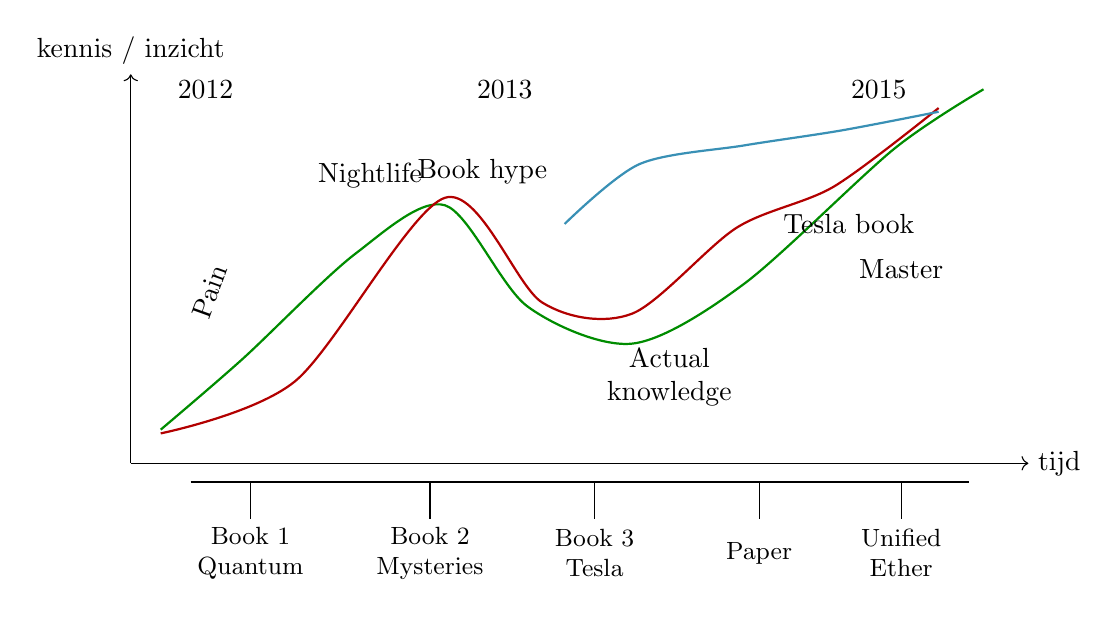
\begin{tikzpicture}[scale=0.95]
  \draw[->] (0,0) -- (12,0) node[right]{tijd};
  \draw[->] (0,0) -- (0,5.2) node[above]{kennis / inzicht};
  \node at (1,5.0) {2012};
  \node at (5,5.0) {2013};
  \node at (10,5.0) {2015};
  \draw[thick,green!55!black,smooth] plot coordinates {(0.4,0.45) (1.5,1.4) (3,2.8) (4.2,3.45) (5.3,2.1) (6.7,1.6) (8.2,2.4) (10.2,4.2) (11.4,5.0)};
  \draw[thick,red!70!black,smooth] plot coordinates {(0.4,0.4) (2.2,1.1) (4.2,3.55) (5.5,2.15) (6.7,2.0) (8.1,3.15) (9.4,3.7) (10.8,4.75)};
  \draw[thick,cyan!70!black,smooth] plot coordinates {(5.8,3.2) (6.8,4.0) (8.2,4.25) (9.5,4.45) (10.8,4.7)};
  \node[align=center,rotate=70] at (1.05,2.3) {Pain};
  \node[align=center] at (3.2,3.85) {Nightlife};
  \node[align=center] at (4.7,3.9) {Book hype};
  \node[align=center] at (7.2,1.15) {Actual\\knowledge};
  \node[align=center] at (9.6,3.2) {Tesla book};
  \node[align=center] at (10.3,2.6) {Master};
  \draw (0.8,-0.25) -- (11.2,-0.25);
  \foreach \x/\txt in {1.6/{Book 1\\Quantum},4.0/{Book 2\\Mysteries},6.2/{Book 3\\Tesla},8.4/{Paper},10.3/{Unified\\Ether}} {
    \draw (\x,-0.25) -- (\x,-0.75);
    \node[align=center,font=\small] at (\x,-1.2) {\txt};
  }
\end{tikzpicture}
\end{center}

Onderaan staat een tweede schets met de tegenstelling tussen waargenomen en werkelijke kennis:

$$
\text{``I think you know''} \quad \longrightarrow \quad
\text{``I know that I don't know''}.
$$

\begin{center}
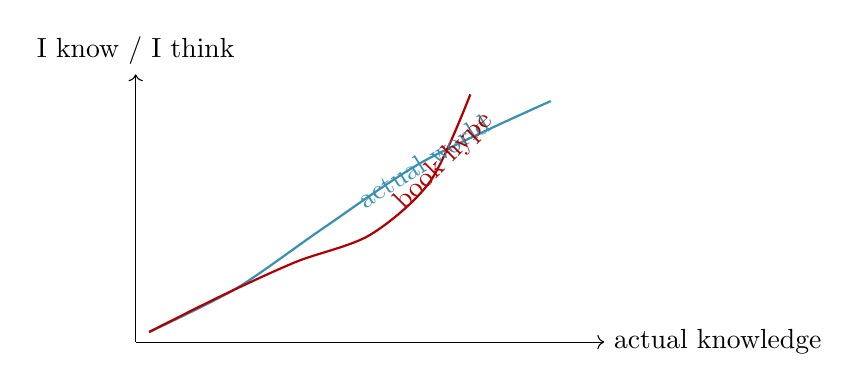
\begin{tikzpicture}[scale=0.85]
  \draw[->] (0,0) -- (7,0) node[right]{actual knowledge};
  \draw[->] (0,0) -- (0,4) node[above]{I know / I think};
  \draw[thick,cyan!70!black,smooth] plot coordinates {(0.2,0.15) (1.5,0.8) (2.8,1.7) (4.3,2.7) (6.2,3.6)};
  \draw[thick,red!70!black,smooth] plot coordinates {(0.2,0.15) (1.3,0.7) (2.4,1.2) (3.5,1.6) (4.4,2.4) (5.0,3.7)};
  \node[cyan!70!black,rotate=32] at (4.3,2.7) {actual world};
  \node[red!70!black,rotate=45] at (4.6,2.7) {book hype};
\end{tikzpicture}
\end{center}

\newpage

\section*{Pagina 2 --- Flower of Life en metafysische notities}
Schematische ``Flower of Life''-constructie:

\begin{center}
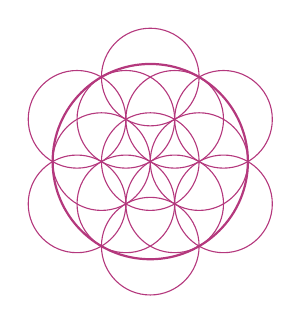
\begin{tikzpicture}[scale=0.62]
  \foreach \x/\y in {0/0,1/0,-1/0,0.5/0.866,-0.5/0.866,0.5/-0.866,-0.5/-0.866,1.5/0.866,-1.5/0.866,1.5/-0.866,-1.5/-0.866,0/1.732,0/-1.732} {
    \draw[magenta!70!black,thin] (\x,\y) circle (1);
  }
  \draw[magenta!70!black,thick] (0,0) circle (2);
\end{tikzpicture}
\end{center}

Tekstuele notitie onderaan de pagina:

\begin{quote}
Zwaartekracht is de aantrekking tot licht.\\
Licht reist niet.\\
Alle materie in beweging zoekt naar rust.\\
Licht = rust.
\end{quote}

In compacte vorm:

$$
\text{zwaartekracht} \sim \text{aantrekking tot licht},
\qquad
\text{licht} = \text{rust}.
$$

\newpage

\section*{Pagina 3 --- Maxwell, divergentie, rotatie en Laplace}
Bovenaan staat een overzicht van Maxwell-vergelijkingen in integrale en differentiële vorm.

$$
\begin{aligned}
\oint_{\partial V} \vect{E}\cdot \dd \vect{A}
    &= \frac{q}{\varepsilon_0},\\
\oint_{\partial V} \vect{B}\cdot \dd \vect{A}
    &= 0,\\
\oint_{\partial A} \vect{E}\cdot \dd \vect{l}
    &= -\frac{\partial \Phi_B}{\partial t},\\
\oint_{\partial A} \vect{B}\cdot \dd \vect{l}
    &= \mu_0 I+\mu_0\varepsilon_0\frac{\partial \Phi_E}{\partial t}.
\end{aligned}
$$

$$
\begin{aligned}
\nabla\cdot\vect{E} &= \frac{\rho}{\varepsilon_0},\\
\nabla\cdot\vect{B} &= 0,\\
\nabla\times\vect{E} &= -\frac{\partial \vect{B}}{\partial t},\\
\nabla\times\vect{B} &= \mu_0\left(\vect{J}+\varepsilon_0\frac{\partial \vect{E}}{\partial t}\right).
\end{aligned}
$$

Divergentie van een vectorveld $\vect{V}$:

$$
\nabla\cdot\vect{V}
=
\frac{\partial V_x}{\partial x}
+
\frac{\partial V_y}{\partial y}
+
\frac{\partial V_z}{\partial z}.
$$

Stelling van Gauss en Stokes:

$$
\int_V \nabla\cdot\vect{v}\,\dd V
=
\oint_{\partial V} \vect{v}\cdot\vect{n}\,\dd A,
\qquad
\oint_{\partial A}\vect{v}\cdot\dd\vect{l}
=
\int_A\left(\nabla\times\vect{v}\right)\cdot\vect{n}\,\dd A.
$$

Curl in cartesische coördinaten:

$$
\nabla\times\vect{v}
=
\left(\frac{\partial v_z}{\partial y}-\frac{\partial v_y}{\partial z}\right)\hat{\vect{x}}
+
\left(\frac{\partial v_x}{\partial z}-\frac{\partial v_z}{\partial x}\right)\hat{\vect{y}}
+
\left(\frac{\partial v_y}{\partial x}-\frac{\partial v_x}{\partial y}\right)\hat{\vect{z}}.
$$

Gradient en Laplace-operator:

$$
\nabla \zeta
=
\frac{\partial \zeta}{\partial x}\hat{\vect{x}}
+
\frac{\partial \zeta}{\partial y}\hat{\vect{y}}
+
\frac{\partial \zeta}{\partial z}\hat{\vect{z}},
\qquad
\nabla^2 V
=
\frac{\partial^2 V}{\partial x^2}
+
\frac{\partial^2 V}{\partial y^2}
+
\frac{\partial^2 V}{\partial z^2}.
$$

\newpage

\section*{Pagina 4 --- vortex, circulatie en energie}
Circulatie als flux van vorticiteit door een oppervlak:

$$
\Gamma
=
\oint_{\partial A} \vect{u}\cdot\dd\vect{s}
=
\int_A \bm{\omega}\cdot\vect{n}\,\dd A.
$$

De notitie onderscheidt drie bijdragen aan vorticiteit:

\begin{itemize}
  \item absolute vorticiteit;
  \item relatieve vorticiteit;
  \item planetaire vorticiteit.
\end{itemize}

In compacte vorm:

$$
\zeta_a=\zeta+f.
$$

De pagina bevat een box met behoudsvorm:

$$
\frac{\partial \Gamma}{\partial t}=0,
\qquad
\frac{\partial(\zeta+f)}{\partial t}=0
\quad
\text{voor een sterk vereenvoudigd geval}.
$$

Een algemene circulatievergelijking wordt schematisch genoteerd als:

$$
\frac{D\Gamma}{Dt}
=
\oint \frac{\dd p}{\rho}
+
\oint \vect{G}\cdot\dd\vect{r}
+
\oint \frac{\mu}{\rho}\nabla^2\vect{v}\cdot\dd\vect{r}.
$$

Hierbij zijn de labels in de notitie ongeveer:

\begin{itemize}
  \item verandering van circulatie;
  \item barokliene of drukterm;
  \item lichaamskracht;
  \item fysische of viskeuze kracht.
\end{itemize}

Onderaan staat een Bernoulli-achtige energievoorwaarde:

$$
\vect{v}\times\bm{\omega}
=
\frac{1}{\rho}\nabla P,
$$

met totale druk of energiehoogte:

$$
P_e
=
P+\frac{1}{2}\rho V^2+\rho U.
$$

\newpage

\section*{Pagina 5 --- vorticiteit als rotatie van snelheid}
De pagina start met de relatie tussen hoekrotatie en de curl van het snelheidsveld:

$$
\bm{\omega}
=
\frac{1}{2}\left(\nabla\times\vect{V}\right).
$$

Uitgeschreven in determinantvorm:

$$
\bm{\omega}
=
\frac{1}{2}
\begin{vmatrix}
\hat{\vect{x}}_1 & \hat{\vect{x}}_2 & \hat{\vect{x}}_3\\
\frac{\partial}{\partial x_1} & \frac{\partial}{\partial x_2} & \frac{\partial}{\partial x_3}\\
V_{x_1} & V_{x_2} & V_{x_3}
\end{vmatrix}.
$$

Componentvorm:

$$
\begin{aligned}
\bm{\omega}
&=
\frac{1}{2}
\left(\frac{\partial V_{x_3}}{\partial x_2}
      -\frac{\partial V_{x_2}}{\partial x_3}\right)\hat{\vect{x}}_1\\
&\quad+
\frac{1}{2}
\left(\frac{\partial V_{x_1}}{\partial x_3}
      -\frac{\partial V_{x_3}}{\partial x_1}\right)\hat{\vect{x}}_2\\
&\quad+
\frac{1}{2}
\left(\frac{\partial V_{x_2}}{\partial x_1}
      -\frac{\partial V_{x_1}}{\partial x_2}\right)\hat{\vect{x}}_3.
\end{aligned}
$$

Voor een viskeuze puntwervel of Lamb--Oseen-achtige vortex staat:

$$
V_\theta(R,t)
=
\frac{\Gamma}{2\pi R}
\left(
1-\exp\left(-\frac{R^2}{4\nu t}\right)
\right),
\qquad
R_c\sim\sqrt{4\nu t}.
$$

\newpage

\section*{Pagina 6 --- veldoperatoren en vectoridentiteiten}
Vectorveld:

$$
\vect{A}
=
A_x\hat{\vect{x}}
+
A_y\hat{\vect{y}}
+
A_z\hat{\vect{z}}.
$$

Gradient:

$$
\nabla V
=
\hat{\vect{x}}\frac{\partial V}{\partial x}
+
\hat{\vect{y}}\frac{\partial V}{\partial y}
+
\hat{\vect{z}}\frac{\partial V}{\partial z}.
$$

Divergentie:

$$
\nabla\cdot\vect{A}
=
\frac{\partial A_x}{\partial x}
+
\frac{\partial A_y}{\partial y}
+
\frac{\partial A_z}{\partial z}.
$$

Curl:

$$
\nabla\times\vect{A}
=
\left(\frac{\partial A_z}{\partial y}-\frac{\partial A_y}{\partial z}\right)\hat{\vect{x}}
+
\left(\frac{\partial A_x}{\partial z}-\frac{\partial A_z}{\partial x}\right)\hat{\vect{y}}
+
\left(\frac{\partial A_y}{\partial x}-\frac{\partial A_x}{\partial y}\right)\hat{\vect{z}}.
$$

Laplace:

$$
\Delta A
=
\nabla^2 A
=
\frac{\partial^2 A}{\partial x^2}
+
\frac{\partial^2 A}{\partial y^2}
+
\frac{\partial^2 A}{\partial z^2}.
$$

Identiteiten uit de rechterbox:

$$
\begin{aligned}
\nabla\cdot(\nabla\times\vect{A}) &= 0,\\
\vect{A}\times\vect{B} &= -\vect{B}\times\vect{A},\\
\nabla\cdot(\vect{A}\times\vect{B})
&=
\vect{B}\cdot(\nabla\times\vect{A})
-
\vect{A}\cdot(\nabla\times\vect{B}),\\
\nabla\times(\vect{A}\times\vect{B})
&=
(\vect{B}\cdot\nabla)\vect{A}
-\vect{B}(\nabla\cdot\vect{A})
-(\vect{A}\cdot\nabla)\vect{B}
+\vect{A}(\nabla\cdot\vect{B}),\\
\vect{A}\cdot(\vect{B}\times\vect{C})
&=
\vect{B}\cdot(\vect{C}\times\vect{A})
=
\vect{C}\cdot(\vect{A}\times\vect{B}).
\end{aligned}
$$

\newpage

\section*{Pagina 7 --- straling, temperatuur en Planck}
De pagina bevat een afleiding rond energie, temperatuur en spectrale straling. Bovenaan:

$$
E=\frac{R}{N}T,
$$

waarbij $\frac{R}{N}=k_B$ de Boltzmannconstante voorstelt.

Relatie tussen energiedichtheid en spectrale dichtheid:

$$
E_\nu
=
\frac{c^3}{8\pi\nu^2}P_\nu.
$$

Daaruit volgt in de Rayleigh--Jeans-benadering:

$$
P_\nu\,\dd \nu
=
\frac{8\pi\nu^2}{c^3}\frac{R}{N}T\,\dd \nu.
$$

De integraal divergeert:

$$
\int_0^\infty P_\nu\,\dd\nu
=
\frac{8\pi}{c^3}\frac{R}{N}T
\int_0^\infty \nu^2\,\dd\nu
=
\infty.
$$

Planck-vorm:

$$
P_\nu
=
\frac{A\nu^3}{e^{B\nu/T}-1}.
$$

Genoteerde constantewaarden:

$$
A \approx \onzeker{6.10\times10^{-36}},
\qquad
B \approx \onzeker{4.866\times10^{-11}}.
$$

De notitie vergelijkt deze vorm met de limiet voor lage frequenties:

$$
P_\nu
\approx
\frac{A}{B}\nu^2 T,
\qquad
\frac{R}{N}
=
\frac{c^3}{8\pi}\frac{A}{B}
\quad
\text{of equivalent volgens notatiekeuze}.
$$

\newpage

\section*{Pagina 8 --- bulkmodulus, geluidssnelheid en veerstijfheid}
Bulkmodulus:

$$
K=-V\frac{\partial P}{\partial V}.
$$

Met dichtheid $\rho$:

$$
K=\rho\frac{\partial P}{\partial \rho}.
$$

Voor geluidssnelheid in een medium:

$$
c=\sqrt{\frac{K}{\rho}}.
$$

Er staan ook analoge veer- en rotatiestijfheden:

$$
k=\frac{F}{s},
\qquad
\kappa=\frac{m}{\phi}.
$$

Interpretatie volgens de labels:

\begin{itemize}
  \item $K$: weerstand tegen compressie;
  \item $k$: lineaire veerstijfheid;
  \item $\kappa$: torsie- of rotatiestijfheid.
\end{itemize}

\newpage

\section*{Pagina 9 --- relatieve, planetaire en potentiële vorticiteit}
Voor een horizontaal snelheidsveld $\vect{V}=(u,v)$:

$$
\zeta
=
\frac{\partial v}{\partial x}
-
\frac{\partial u}{\partial y}.
$$

In natuurlijke coördinaten verschijnt een krommingsterm:

$$
\zeta
=
-\frac{\partial V}{\partial n}
+
\frac{V}{R}.
$$

De notitie benoemt:

$$
\zeta_p
=
2\Omega\sin\varphi
=
f,
$$

$$
\zeta_a
=
\zeta+f.
$$

In een vereenvoudigde behoudsvorm:

$$
\frac{\partial(\zeta+f)}{\partial t}=0.
$$

Potentiële vorticiteit wordt aangeduid als:

$$
\Pi
=
\frac{\zeta+f}{h},
$$

waarbij de handgeschreven notitie op de pagina bij $\Pi$ deels is doorgestreept.

\newpage

\section*{Pagina 10 --- natuurlijke coördinaten}
De snelheid is ontbonden langs een raakrichting $\hat{\vect{s}}$ en een normaalrichting $\hat{\vect{n}}$.

$$
\hat{\vect{s}}
=
(\cos\varphi,\sin\varphi),
\qquad
\hat{\vect{n}}
=
(-\sin\varphi,\cos\varphi).
$$

Componenten:

$$
u
=
V\hat{s}_x
=
V\cos\varphi,
\qquad
v
=
V\hat{s}_y
=
V\sin\varphi.
$$

Relaties tussen normaal en raakvector:

$$
\hat{n}_x=-\hat{s}_y,
\qquad
\hat{n}_y=\hat{s}_x.
$$

Afgeleiden van de richting:

$$
\frac{\partial \hat{s}_y}{\partial x}
=
\cos\varphi\frac{\partial\varphi}{\partial x}
=
\hat{s}_x\frac{\partial\varphi}{\partial x},
$$

$$
\frac{\partial \hat{s}_x}{\partial y}
=
-\sin\varphi\frac{\partial\varphi}{\partial y}
=
-\hat{s}_y\frac{\partial\varphi}{\partial y}.
$$

Daaruit:

$$
\frac{\partial \hat{s}_y}{\partial x}
-
\frac{\partial \hat{s}_x}{\partial y}
=
\hat{s}_x\frac{\partial\varphi}{\partial x}
+
\hat{s}_y\frac{\partial\varphi}{\partial y}
=
\frac{\dd\varphi}{\dd s}
=
\frac{1}{R}.
$$

\newpage

\section*{Pagina 11 --- momentumformule en start vorticiteitsvergelijking}
Algemene impulsvergelijking in $x$-richting:

$$
\rho
\left(
\frac{\partial u}{\partial t}
+
u\frac{\partial u}{\partial x}
+
v\frac{\partial u}{\partial y}
+
w\frac{\partial u}{\partial z}
-
fv
\right)
=
-\frac{\partial p}{\partial x}
+
R_x.
$$

Hydrostatische benadering:

$$
\frac{\partial p}{\partial z}=-\rho g.
$$

Horizontale componenten:

$$
\begin{aligned}
\rho
\left(
\frac{\partial u}{\partial t}
+
u\frac{\partial u}{\partial x}
+
v\frac{\partial u}{\partial y}
-
fv
\right)
&=
-\frac{\partial p}{\partial x}+R_x,\\
\rho
\left(
\frac{\partial v}{\partial t}
+
u\frac{\partial v}{\partial x}
+
v\frac{\partial v}{\partial y}
+
fu
\right)
&=
-\frac{\partial p}{\partial y}+R_y.
\end{aligned}
$$

De pagina geeft een schets waarin stroming van hoge druk naar lage druk loopt. De relatieve vorticiteit wordt opnieuw genoteerd als:

$$
\zeta
=
\frac{\partial v}{\partial x}
-
\frac{\partial u}{\partial y}.
$$

Door de $x$-impulsvergelijking naar $y$ en de $y$-impulsvergelijking naar $x$ te differentiëren ontstaat de vorticiteitsvergelijking op de volgende pagina.

\newpage

\section*{Pagina 12 --- vorticiteitsformule in componenten}
De centrale box geeft de horizontale vorticiteitsvergelijking:

$$
\begin{aligned}
\frac{\partial \zeta}{\partial t}
+
u\frac{\partial \zeta}{\partial x}
+
v\frac{\partial \zeta}{\partial y}
+
(\zeta+f)
\left(
\frac{\partial u}{\partial x}
+
\frac{\partial v}{\partial y}
\right)
+
\beta v
=
\frac{\partial R_y}{\partial x}
-
\frac{\partial R_x}{\partial y}.
\end{aligned}
$$

Labels op de pagina:

\begin{itemize}
  \item $\frac{\partial \zeta}{\partial t}$: lokale verandering;
  \item $u\frac{\partial \zeta}{\partial x}+v\frac{\partial \zeta}{\partial y}$: horizontale advectie;
  \item $(\zeta+f)\left(\frac{\partial u}{\partial x}+\frac{\partial v}{\partial y}\right)$: strekking;
  \item $\beta v$: beta-effect;
  \item rechterlid: wrijving of externe kracht.
\end{itemize}

Onderaan wordt het wrijvingsterm-notatieblok genoteerd als:

$$
B_v
=
\frac{\partial R_y}{\partial x}
-
\frac{\partial R_x}{\partial y}.
$$

Een tussenvorm onderaan is deels zwak leesbaar:

$$
\onzeker{
\frac{\partial R_y}{\partial x}
-
\frac{\partial R_x}{\partial y}
\approx
-g\frac{\partial^2 h}{\partial x\,\partial y}
+
\frac{\partial R_y}{\partial x}
}.
$$

\newpage

\section*{Pagina 13 --- incompressibele stroming en potentiaalstroming}
Continuïteitsvergelijking voor incompressibele stroming:

$$
\frac{\partial u}{\partial x}
+
\frac{\partial v}{\partial y}
+
\frac{\partial w}{\partial z}
=
0.
$$

Irrotationaliteit:

$$
\nabla\times\vect{v}=0.
$$

Als het snelheidsveld uit een potentiaal komt:

$$
\vect{v}=\nabla\phi,
$$

dan volgt uit incompressibiliteit:

$$
\nabla\cdot\vect{v}
=
\nabla\cdot\nabla\phi
=
\nabla^2\phi
=
0.
$$

In de rechterbox wordt een algemene impulsvergelijking genoteerd:

$$
\rho\frac{\partial \vect{u}}{\partial t}
+
\rho(\vect{v}\cdot\nabla)\vect{u}
=
-\nabla p
+
\nu\nabla^2\vect{u}
+
\onzeker{\text{extra term}}.
$$

Voor vorticiteit verschijnt schematisch:

$$
\rho\frac{\partial\bm{\omega}}{\partial t}
+
\rho(\vect{v}\cdot\nabla)\bm{\omega}
=
\onzeker{\bm{\omega}\cdot\nabla\vect{v}}
+
\nu\nabla^2\bm{\omega}.
$$

Onderaan staat een schets van een waterkolom met bodem $z=0$ en oppervlak $z=\eta$.

\newpage

\section*{Pagina 14 --- dieptegemiddelde continuïteit}
Deze pagina leidt een ondiepwater-continuïteitsvorm af. De centrale eindvorm is:

$$
\frac{Dh}{Dt}
+
h
\left(
\frac{\partial u}{\partial x}
+
\frac{\partial v}{\partial y}
\right)
=
0.
$$

Equivalent:

$$
\frac{\partial h}{\partial t}
+
u\frac{\partial h}{\partial x}
+
v\frac{\partial h}{\partial y}
+
h
\left(
\frac{\partial u}{\partial x}
+
\frac{\partial v}{\partial y}
\right)
=
0.
$$

Daaruit volgt:

$$
\frac{\partial u}{\partial x}
+
\frac{\partial v}{\partial y}
=
-\frac{1}{h}\frac{Dh}{Dt}.
$$

De handgeschreven marge bevat losse notities over druk, wrijving en de voorwaarde dat bij $\zeta=0$ of $T=0$ geen vorticiteit zal ontstaan. Deze tekst is deels onleesbaar.

\newpage

\section*{Pagina 15 --- potentiële vorticiteitsformule}
Startpunt is de diepte-geïntegreerde continuïteit:

$$
\frac{\partial u}{\partial x}
+
\frac{\partial v}{\partial y}
=
-\frac{1}{h}\frac{Dh}{Dt}.
$$

Invullen in de vorticiteitsformule geeft:

$$
\frac{D\zeta}{Dt}
+
(\zeta+f)
\left(
\frac{\partial u}{\partial x}
+
\frac{\partial v}{\partial y}
\right)
+
\beta v
=
\frac{\partial R_y}{\partial x}
-
\frac{\partial R_x}{\partial y}.
$$

Met $\frac{Df}{Dt}=\beta v$:

$$
\frac{D(\zeta+f)}{Dt}
-
\frac{\zeta+f}{h}\frac{Dh}{Dt}
=
\frac{\partial R_y}{\partial x}
-
\frac{\partial R_x}{\partial y}.
$$

Delen door $h$ geeft de centrale formule:

$$
\boxed{
\frac{D}{Dt}
\left(
\frac{\zeta+f}{h}
\right)
=
\frac{1}{h}
\left(
\frac{\partial R_y}{\partial x}
-
\frac{\partial R_x}{\partial y}
\right)
}
$$

Zonder wrijving:

$$
\frac{D}{Dt}
\left(
\frac{\zeta+f}{h}
\right)
=
0.
$$

Dus de potentiële vorticiteit blijft behouden:

$$
\Pi
=
\frac{\zeta+f}{h}
=
\text{constant}.
$$

\newpage

\section*{Pagina 16 --- De Broglie en matrixnotatie}
Bovenaan staat ``De Broglie'' met een exponentiële verhouding:

$$
B
=
\frac{R}{r}
=
c_1 e^{6.996\phi}
=
\onzeker{-274.07496}.
$$

De pagina toont schetsen van cirkelvormige banen en een bol/doorsnede. Daarna volgt matrix- en transformatienotatie:

$$
A^{-1}A=I,
\qquad
A\frac{1}{A}=1.
$$

Lineaire transformatie:

$$
x'_i
=
\sum_{k=1}^{N+1}
a_{ik}x_k.
$$

Orthogonaliteitsachtige relatie:

$$
\sum_k a_{ik}a_{\ell k}
=
\sum_k a_{ki}a_{k\ell}
\quad
\onzeker{\text{notatie deels onzeker}}.
$$

Marge:

$$
\onzeker{\text{Clifford}=\text{Real Numbers}}.
$$

\newpage

\section*{Pagina 17 --- vorticiteit en circulatie}
Definitie van vorticiteit:

$$
\bm{\omega}
=
\nabla\times\vect{V}.
$$

Definitie van circulatie rond een gesloten kromme:

$$
C
=
\oint \vect{V}\cdot\dd\vect{l}.
$$

Met Stokes:

$$
C
=
\int_A \bm{\omega}\cdot\dd\vect{S}.
$$

Lokale vorm:

$$
\hat{\vect{n}}\cdot(\nabla\times\vect{V})
=
\lim_{A\to 0}
\frac{1}{A}
\oint_{\partial A}\vect{V}\cdot\dd\vect{l}.
$$

Vast-lichaam-rotatie:

$$
u_\theta=\Omega r,
\qquad
\bm{\omega}=\nabla\times\vect{V}=\omega_z\hat{\vect{k}}.
$$

In cilindrische coördinaten:

$$
\omega_z
=
\frac{1}{r}
\frac{\partial}{\partial r}
(r u_\theta)
-
\frac{1}{r}\frac{\partial u_r}{\partial \theta}.
$$

Voor $u_\theta=\Omega r$ en $u_r=0$:

$$
\omega_z
=
\frac{1}{r}\frac{\partial}{\partial r}(\Omega r^2)
=
2\Omega.
$$

Irrotationele vortex:

$$
u_\theta=\frac{\kappa}{r},
\qquad
\omega_z
=
\frac{1}{r}\frac{\partial}{\partial r}(\kappa)
=
0.
$$

\newpage

\section*{Pagina 18 --- vorticiteit in een draaiend referentiekader}
Voor een draaiend referentiekader staat de vorticiteitsvergelijking schematisch als:

$$
\frac{D\bm{\omega}_a}{Dt}
=
\left((\bm{\omega}+2\bm{\Omega})\cdot\nabla\right)\vect{V}
-
(\bm{\omega}+2\bm{\Omega})(\nabla\cdot\vect{V})
+
\frac{1}{\rho^2}
(\nabla\rho\times\nabla p).
$$

Een equivalente vorm per massa:

$$
\frac{D}{Dt}
\left(
\frac{\bm{\omega}}{\rho}
\right)
=
\left(
\frac{\bm{\omega}+2\bm{\Omega}}{\rho}
\cdot\nabla
\right)\vect{V}
+
\frac{1}{\rho^3}
(\nabla\rho\times\nabla p).
$$

De schetsen tonen het uittrekken van vortexlijnen: bij verticale strekking wordt vorticiteit versterkt.

Een genoteerde transportvorm voor een vorticiteitscomponent:

$$
\frac{D\zeta}{Dt}
=
-\frac{\partial u_r}{\partial z}
+
\nu\nabla^2\zeta
\quad
\onzeker{\text{componentnotatie onzeker}}.
$$

Onderaan staat een exponentiële vortexprofielvorm:

$$
G
=
G_0\exp\left(-\frac{k r^2}{4\nu}\right),
\qquad
r_0
=
2\sqrt{\frac{\nu}{\lambda}}
\quad
\onzeker{\text{parameters uit notitie}}.
$$

\newpage

\section*{Pagina 19 --- radiale convergentie en vortexbalans}
De schets toont een verticale vortex met radiale convergentie en opwaartse beweging.

Genoteerd snelheidsveld:

$$
\vect{V}
=
\left(
-\frac{1}{2}\alpha r,\;
U_\theta,\;
\alpha z
\right),
$$

met radiale convergentie, swirl en verticale uitzetting.

Massabehoud in cilindrische coördinaten:

$$
\nabla\cdot\vect{V}
=
\frac{1}{r}\frac{\partial}{\partial r}(rV_r)
+
\frac{1}{r}\frac{\partial V_\theta}{\partial\theta}
+
\frac{\partial V_z}{\partial z}.
$$

Voor axisymmetrie en $V_r=-\frac{1}{2}\alpha r$, $V_z=\alpha z$:

$$
\nabla\cdot\vect{V}
=
\frac{1}{r}\frac{\partial}{\partial r}
\left(-\frac{1}{2}\alpha r^2\right)
+
\alpha
=
-\alpha+\alpha
=
0.
$$

Vorticiteitscomponenten worden genoteerd als:

$$
\begin{aligned}
\omega_\theta
&=
\frac{\partial V_r}{\partial z}
-
\frac{\partial V_z}{\partial r}
=
0,\\
\omega_r
&=
\frac{1}{r}\frac{\partial V_z}{\partial\theta}
-
\frac{\partial V_\theta}{\partial z}
=
0,\\
\omega_z
&=
\frac{1}{r}\frac{\partial(rV_\theta)}{\partial r}
-
\frac{1}{r}\frac{\partial V_r}{\partial\theta}.
\end{aligned}
$$

Marge:

\begin{quote}
De start van $u_\theta$ moet de balans brengen.
\end{quote}

\newpage

\section*{Pagina 20 --- vectorcalculus in cartesische coördinaten}
Vector in basisnotatie:

$$
\vect{y}
=
\sum_i V_i\vect{e}_i.
$$

Tweederangstensor:

$$
\vect{T}
=
\sum_i\sum_j
T_{ij}\vect{e}_i\vect{e}_j.
$$

Inproduct:

$$
\vect{A}\cdot\vect{B}
=
A_1B_1+A_2B_2+A_3B_3
=
\sum_{i=1}^{3}A_iB_i.
$$

Met Kronecker-delta:

$$
\vect{e}_i\cdot\vect{e}_j
=
\delta_{ij},
\qquad
\delta_{ij}
=
\begin{cases}
1, & i=j,\\
0, & i\neq j.
\end{cases}
$$

Componentvorm van het inproduct:

$$
A_iB_j\delta_{ij}
=
A_iB_i.
$$

Uitproduct met Levi-Civita-symbool:

$$
\vect{A}\times\vect{B}
=
\varepsilon_{ijk}A_jB_k\,\vect{e}_i.
$$

De pagina bevat daarnaast een kleine assenschets met cartesische coördinaten en vectorbasis $\vect{e}_1,\vect{e}_2,\vect{e}_3$.

\clearpage
\section*{Bundel: pagina's 21--40}
\section*{Pagina 21 -- Opgave Navier--Stokes}

\onzeker{De titel lijkt te verwijzen naar ``opgaven de Navier--Stokes te bewijzen''.}

\begin{enumerate}[label=\alph*)]
    \item Kies een cilindrisch coördinatenstelsel.
    \item Neem \onzeker{de meridiaan/doorsnede} als uitgangspunt.
    \item Voor alle velden wordt de snelheid beschreven door
    \[
        \mathbf{v}
        =
        v_r\,\mathbf{e}_r
        +
        v_\theta\,\mathbf{e}_\theta
        +
        v_z\,\mathbf{e}_z .
    \]
    \item Gevraagde grootheden:
    \[
        p,\qquad \mathbf{v},\qquad \bm{\omega}=\curl\mathbf{v}.
    \]
    \item De oplossing moet voldoen aan de juiste randvoorwaarden en aan behoud van massa.
\end{enumerate}

\section*{Pagina 22 -- Stationaire, langzame stroming rond een cilinder}

\onzeker{De bovenregel lijkt: ``Vind de snelheid verdeling'' voor stroming rond een cilinder.}

We kiezen cilindercoördinaten $(r,\theta,z)$ en nemen een stationaire stroming:
\[
    \frac{\p}{\p t}=0 .
\]

Voor een tweedimensionale stroming geldt:
\[
    \mathbf{v}=v_r(r,\theta)\,\mathbf{e}_r
    +
    v_\theta(r,\theta)\,\mathbf{e}_\theta,
    \qquad
    v_z=0 .
\]

Randvoorwaarden, zoals in de notities aangeduid:
\begin{align*}
    \mathbf{v}(r=R) &= \mathbf{0},\\
    \mathbf{v}(r\to\infty) &\to U_\infty\,\mathbf{e}_x .
\end{align*}

In cilindercoördinaten kan de ver-stroom worden geschreven als
\[
    U_\infty\,\mathbf{e}_x
    =
    U_\infty\cos\theta\,\mathbf{e}_r
    -
    U_\infty\sin\theta\,\mathbf{e}_\theta .
\]

\section*{Pagina 23 -- Randvoorwaarden en behoudswetten}

\onzeker{Deze pagina lijkt de behoudswetten en randvoorwaarden voor de cilinderopgave te combineren.}

Voor oncompressibele stroming:
\[
    \diver \mathbf{v}=0 .
\]

Voor stationaire viscositeit-dominante stroming:
\[
    -\grad p+\mu \nabla^2\mathbf{v}=\mathbf{0}.
\]

Componenten:
\begin{align*}
    v_r(R,\theta)&=0, &
    v_\theta(R,\theta)&=0,\\
    v_r(\infty,\theta)&=U_\infty\cos\theta, &
    v_\theta(\infty,\theta)&=-U_\infty\sin\theta.
\end{align*}

Met \onzeker{een constante druk op grote afstand}:
\[
    p(r\to\infty)=p_\infty .
\]

\section*{Pagina 24 -- Navier--Stokes in cilindercoördinaten}

\onzeker{De pagina bevat een reeks componentvergelijkingen; de exacte handgeschreven tekens zijn deels niet leesbaar.}

De continuïteitsvergelijking:
\[
    \frac{1}{r}\frac{\p}{\p r}\left(r v_r\right)
    +
    \frac{1}{r}\frac{\p v_\theta}{\p\theta}
    +
    \frac{\p v_z}{\p z}
    =
    0 .
\]

Radiale impulsvergelijking:
\begin{align*}
\rho\left(
    \frac{\p v_r}{\p t}
    +
    v_r\frac{\p v_r}{\p r}
    +
    \frac{v_\theta}{r}\frac{\p v_r}{\p\theta}
    +
    v_z\frac{\p v_r}{\p z}
    -
    \frac{v_\theta^2}{r}
\right)
&=
-\frac{\p p}{\p r}
+
\mu\left(
\nabla^2 v_r
-
\frac{v_r}{r^2}
-
\frac{2}{r^2}\frac{\p v_\theta}{\p\theta}
\right).
\end{align*}

Azimutale impulsvergelijking:
\begin{align*}
\rho\left(
    \frac{\p v_\theta}{\p t}
    +
    v_r\frac{\p v_\theta}{\p r}
    +
    \frac{v_\theta}{r}\frac{\p v_\theta}{\p\theta}
    +
    v_z\frac{\p v_\theta}{\p z}
    +
    \frac{v_r v_\theta}{r}
\right)
&=
-\frac{1}{r}\frac{\p p}{\p\theta}
+
\mu\left(
\nabla^2 v_\theta
-
\frac{v_\theta}{r^2}
+
\frac{2}{r^2}\frac{\p v_r}{\p\theta}
\right).
\end{align*}

\section*{Pagina 25 -- Schets en lokale componenten}

\onzeker{De pagina bevat vooral een schets met lokale richtingen en korte notaties.}

Vermoedelijke componentnotatie:
\[
    \mathbf{v}
    =
    v_r\,\mathbf{e}_r
    +
    v_\theta\,\mathbf{e}_\theta .
\]

Voor rotatie:
\[
    \omega_z
    =
    \left(\curl\mathbf{v}\right)_z
    =
    \frac{1}{r}\frac{\p}{\p r}\left(r v_\theta\right)
    -
    \frac{1}{r}\frac{\p v_r}{\p\theta}.
\]

\section*{Pagina 26 -- Resonantie/schets}

\onzeker{Bovenaan staat mogelijk ``tuning'' of ``turning''; het grootste deel van de pagina is een geometrische schets.}

Een getekende cirkelboog met hoek $\alpha$ en een straal $R$ lijkt te verwijzen naar:
\[
    s=R\alpha .
\]

Verder is genoteerd:
\[
    \onzeker{90^\circ}
    \qquad\text{en}\qquad
    \onzeker{A_r\ \text{of}\ A_\theta}.
\]

\section*{Pagina 27 -- Geometrische schets}

\onzeker{Deze pagina is nagenoeg volledig grafisch. De tekst is niet betrouwbaar leesbaar.}

De schets lijkt de baan van een deeltje of veldlijn te tonen. Een generieke parametrisatie is:
\[
    \mathbf{x}(s)
    =
    x(s)\,\mathbf{e}_x
    +
    y(s)\,\mathbf{e}_y ,
\]
met raakvector:
\[
    \mathbf{t}
    =
    \frac{\dd \mathbf{x}}{\dd s}.
\]

\section*{Pagina 28 -- Veldlijnen / stromingsschets}

\onzeker{Ook deze pagina bestaat hoofdzakelijk uit gekruiste lijnen en pijlen.}

Mogelijke notatie bij de schets:
\[
    \mathbf{v}
    =
    \frac{\dd \mathbf{x}}{\dd t},
    \qquad
    \mathbf{a}
    =
    \frac{\dd \mathbf{v}}{\dd t}.
\]

\section*{Pagina 29 -- Newton}

Er staat duidelijk ``Newton'' bovenaan. De notitie lijkt een krachtenbalans te introduceren:
\[
    \sum \mathbf{F}=m\mathbf{a}.
\]

In differentiaalvorm:
\[
    \dd \mathbf{F}
    =
    \mathbf{T}\,\dd A
    \qquad\text{en}\qquad
    \mathbf{T}=\bm{\sigma}\cdot\mathbf{n}.
\]

\onzeker{De overige symbolen op de pagina zijn grotendeels schetsmatig.}

\section*{Pagina 30 -- Potentiaalstroming}

\onzeker{De pagina vermeldt ``velocity potential'' en bevat formules voor een potentiaal- en stroomfunctie.}

Voor tweedimensionale potentiaalstroming:
\[
    \mathbf{v}=\grad\phi .
\]

Voor oncompressibele stroming:
\[
    \nabla^2 \phi =0 .
\]

Met stroomfunctie $\psi$:
\[
    u=\frac{\p\psi}{\p y},
    \qquad
    v=-\frac{\p\psi}{\p x}.
\]

Complexe potentiaal:
\[
    W(z)=\phi(x,y)+i\psi(x,y),
    \qquad
    z=x+iy .
\]

De notities lijken een constante plus een wervelterm te bevatten:
\[
    W(z)
    =
    U z
    +
    \frac{i\Gamma}{2\pi}\log z
    +
    \onzeker{C}.
\]

\section*{Pagina 31 -- Circulatie in een gesloten contour}

De pagina vermeldt circulatie in een lopende of gesloten contour. De standaardvorm:
\[
    \Gamma
    =
    \oint_C \mathbf{v}\cdot\dd\mathbf{s}.
\]

Volgens Stokes:
\[
    \Gamma
    =
    \iint_A \left(\curl\mathbf{v}\right)\cdot\mathbf{n}\,\dd A
    =
    \iint_A \bm{\omega}\cdot\mathbf{n}\,\dd A .
\]

Voor tweedimensionale stroming:
\[
    \Gamma
    =
    \iint_A \omega_z\,\dd A .
\]

\onzeker{Onderaan lijkt een afleiding te staan voor een vortexsterkte in een contour of wake.}

\section*{Pagina 32 -- Schets van veldlijnen}

\onzeker{Deze pagina is vooral grafisch; er zijn geen betrouwbare losse formules leesbaar.}

De schets wordt genoteerd als een veldlijnvoorstelling:
\[
    \frac{\dd\mathbf{x}}{\dd s}
    \parallel
    \mathbf{v}(\mathbf{x}).
\]

\section*{Pagina 33 -- Schets met mogelijk wervelgebied}

\onzeker{Hoofdzakelijk tekening; fragmenten lijken ``$r$'', ``$R$'' en mogelijk ``$\Gamma$'' te bevatten.}

Een gebruikelijke beschrijving:
\[
    \mathbf{v}_\theta(r)
    =
    \frac{\Gamma}{2\pi r}.
\]

De bijbehorende circulatie:
\[
    \oint_C \mathbf{v}\cdot\dd\mathbf{s}
    =
    2\pi r\,v_\theta
    =
    \Gamma .
\]

\section*{Pagina 34 -- Schets / mogelijke krachtbalans}

\onzeker{De pagina is zeer slecht leesbaar. Er staan meerdere schetsen, pijlen en mogelijk de term $R=F$.}

Een mogelijke balansnotatie:
\[
    \mathbf{R}
    =
    \sum_i \mathbf{F}_i .
\]

Als $R$ een resulterende kracht aanduidt:
\[
    R
    =
    \left\lVert
    \sum_i \mathbf{F}_i
    \right\rVert .
\]

\section*{Pagina 35 -- Fragmentaire schets}

\onzeker{Slechts enkele losse tekens zijn leesbaar. De pagina bevat vermoedelijk een voortzetting van de schets op pagina 34.}

\[
    \onzeker{\text{grafische constructie met } R,\ F,\ \theta}
\]

\section*{Pagina 36 -- Stromingsschets / golfvorm}

\onzeker{De pagina is hoofdzakelijk grafisch met overlappende lijnen.}

Een passende notatie voor een lopende golf of stroomlijn:
\[
    y(x,t)=A\sin(kx-\omega t+\varphi).
\]

\section*{Pagina 37 -- Fragmenten}

\onzeker{Er zijn slechts losse symbolen zichtbaar, waaronder mogelijk $35$ en een pijlrichting.}

\[
    \onzeker{\text{schetsmatige vervolgpagina}}
\]

\section*{Pagina 38 -- Elementaire vorticiteit}

De titel lijkt te verwijzen naar ``elementaire vorticiteit''. Vermoedelijke kern:
\[
    \bm{\omega}
    =
    \curl\mathbf{v}.
\]

Voor een klein oppervlak $\dd A$:
\[
    \dd\Gamma
    =
    \bm{\omega}\cdot\mathbf{n}\,\dd A .
\]

Daaruit:
\[
    \Gamma
    =
    \iint_A \bm{\omega}\cdot\mathbf{n}\,\dd A .
\]

\onzeker{Verder staat er iets over massa en volume in een circulaire doorsnede.}

\section*{Pagina 39 -- Energie / elementen}

\onzeker{De titel lijkt op ``Verenig u elementen'' of ``energie elementen''. De tekst noemt mogelijk elektromagnetisme, speciale relativiteit en coördinaten.}

Genoemde kernwoorden:
\[
    \onzeker{\text{elektromagnetisme}},
    \qquad
    \onzeker{\text{speciale relativiteit}},
    \qquad
    \onzeker{\text{coördinatenstelsel}}.
\]

Mogelijke vectornotatie:
\[
    \mathbf{E},\quad \mathbf{B},\quad
    \mathbf{F}=q\left(\mathbf{E}+\mathbf{v}\times\mathbf{B}\right).
\]

\section*{Pagina 40 -- Circulatie en wervels}

De pagina vermeldt dat vorticiteit de kinematische maat voor rotatie is:
\[
    \bm{\omega}
    =
    \curl\mathbf{v}.
\]

Circulatie is de integraal van de snelheid langs een gesloten kromme:
\[
    C
    =
    \oint_C \mathbf{v}\cdot\dd\mathbf{s}.
\]

Met Stokes:
\[
    C
    =
    \iint_A \bm{\omega}\cdot\mathbf{n}\,\dd A .
\]

Voor een line vortex:
\[
    v_\theta(r)
    =
    \frac{\Gamma}{2\pi r}.
\]

Voor een Rankine-achtige vortex:
\[
    v_\theta(r)
    =
    \begin{cases}
    \Omega r, & r<a,\\
    \dfrac{\Gamma}{2\pi r}, & r>a.
    \end{cases}
\]

Vorticiteit:
\[
    \omega_z
    =
    \frac{1}{r}\frac{\dd}{\dd r}\left(r v_\theta\right).
\]

\clearpage
\section*{Bundel: pagina's 41--60}
\begin{center}
{\Large \textbf{Notebook 2014 -- pagina 41 t/m 60}}\\
\vspace{0.3em}
{\small Hoge-resolutie transcriptie naar \LaTeX. Onduidelijke handgeschreven delen zijn gemarkeerd met \onzeker{...}.}
\end{center}

\section*{Pagina 41 -- vorticiteit in een roterend stelsel}

De pagina bevat een uitbreiding van de vorticiteitsvergelijking met rotatie-termen. De absolute vorticiteit wordt genoteerd als
$$
\omegav_a = \omegav + 2\Omegav .
$$

Een compacte vorm van de genoteerde vergelijking is
$$
\Dt\left(\omegav + 2\Omegav\right)
=
\left(\omegav + 2\Omegav\right)\cdot\grad \V
-
\left(\divergence \V\right)\left(\omegav + 2\Omegav\right)
+
\frac{1}{\rho^2}\grad \rho \times \grad p
+
\nu \grad^2 \omegav .
$$

Voor een incompressibele stroming, met $\divergence\V=0$, blijft
$$
\Dt\left(\omegav + 2\Omegav\right)
=
\left(\omegav + 2\Omegav\right)\cdot\grad \V
+
\frac{1}{\rho^2}\grad \rho \times \grad p
+
\nu \grad^2 \omegav .
$$

Aantekening op de pagina: de vorm wordt gekoppeld aan \onzeker{``momentum in $x,y,z$''} en aan het verschil tussen lokale en materiële verandering.

\section*{Pagina 42 -- tweedimensionale stroming}

Voor een tweedimensionale stroming
$$
\V = u\left(x,y,t\right)\mathbf{e}_x + v\left(x,y,t\right)\mathbf{e}_y
$$
is de enige niet-nul component van de vorticiteit
$$
\omegav = \omega_z \mathbf{e}_z,
\qquad
\omega_z =
\frac{\partial v}{\partial x}
-
\frac{\partial u}{\partial y}.
$$

De continuïteitsvoorwaarde voor incompressibele stroming is
$$
\frac{\partial u}{\partial x}
+
\frac{\partial v}{\partial y}
=0.
$$

Daarom kan een stroomfunctie $\psi$ worden ingevoerd:
$$
u = \frac{\partial \psi}{\partial y},
\qquad
v = -\frac{\partial \psi}{\partial x}.
$$

Hieruit volgt
$$
\omega_z
=
-\left(
\frac{\partial^2 \psi}{\partial x^2}
+
\frac{\partial^2 \psi}{\partial y^2}
\right)
=
-\grad^2\psi.
$$

Equivalent:
$$
\grad^2\psi = -\omega_z.
$$

\section*{Pagina 43 -- Bernoulli en behoud langs een stroomlijn}

De pagina bevat een notitie over \onzeker{Bernoulli} en een schets met doorsneden. De leesbare kern is dat langs een stationaire stroomlijn een energieachtige grootheid constant blijft:
$$
\frac{p}{\rho}
+
\frac{1}{2}\lVert\V\rVert^2
+
gz
=
C.
$$

Bij constante dichtheid kan dit ook als drukvorm worden geschreven:
$$
p
+
\frac{1}{2}\rho \lVert\V\rVert^2
+
\rho gz
=
C.
$$

De schets lijkt een balans over twee doorsneden aan te geven:
$$
A_1 V_1 = A_2 V_2,
\qquad
p_1+\frac{1}{2}\rho V_1^2
=
p_2+\frac{1}{2}\rho V_2^2
\quad
\onzeker{zonder hoogteverschil}.
$$

\section*{Pagina 44 -- stroming rond een obstakel}

Deze pagina bevat vooral schetsen van stroming rond een object en aantekeningen over \onzeker{referentiestelsel / roterende beweging}. De relevante vectornotatie is:
$$
\V =
u\,\mathbf{e}_x + v\,\mathbf{e}_y + w\,\mathbf{e}_z.
$$

Voor een tweedimensionale doorsnede geldt
$$
\V =
u\,\mathbf{e}_x + v\,\mathbf{e}_y,
\qquad
\omegav =
\left(
\frac{\partial v}{\partial x}
-
\frac{\partial u}{\partial y}
\right)\mathbf{e}_z.
$$

De lokale rotatie in een klein materiaal element wordt daarmee gekoppeld aan
$$
\frac{1}{2}\omegav.
$$

\section*{Pagina 45 -- schuine vortex en projecties}

De titel is geïnterpreteerd als \onzeker{``schuine vortex / universum''}. De pagina bevat een 3D-schets met projecties. De algemene notatie past bij een vortexlijn:
$$
\frac{\dd \xvec}{\dd s}
=
\frac{\omegav}{\lVert \omegav\rVert}.
$$

Een vortexlijn voldoet dus aan
$$
\frac{\dd x}{\omega_x}
=
\frac{\dd y}{\omega_y}
=
\frac{\dd z}{\omega_z}.
$$

Voor circulatie rond een gesloten contour $C$:
$$
\Gamma
=
\oint_C \V\cdot \dd\mathbf{l}.
$$

Volgens Stokes:
$$
\Gamma
=
\iint_S
\left(\curl \V\right)\cdot \mathbf{n}\,\dd A
=
\iint_S
\omegav\cdot\mathbf{n}\,\dd A.
$$

\section*{Pagina 46 -- schetsen van gesloten lijnen en rotatie}

De pagina bestaat hoofdzakelijk uit schetsen van gesloten contouren. De formules horen bij circulatie:
$$
C = \oint_{\partial S} \V \cdot \dd\mathbf{l}.
$$

Wanneer $\V$ potentiaal is, $\V=\grad\phi$, dan
$$
\oint_{\partial S}\grad\phi\cdot \dd\mathbf{l}=0
$$
voor enkelvoudig samenhangende gebieden zonder singulariteiten.

Bij een vortexsingulariteit kan echter
$$
\oint_{\partial S}\V\cdot\dd\mathbf{l}=\Gamma
$$
niet nul zijn.

\section*{Pagina 47 -- lijnvortex en circulatie}

De pagina verwijst naar een \onzeker{``1D line vortex''}. De kernnotatie:
$$
\Gamma
=
\oint_C \V\cdot \dd\mathbf{l}.
$$

Voor een zuivere lijnvortex in cilindrische coördinaten:
$$
V_r = 0,
\qquad
V_\theta = \frac{\Gamma}{2\pi r},
\qquad
V_z = 0.
$$

Buiten de kern is
$$
\curl \V = \mathbf{0},
\qquad r>0,
$$
maar rond de singulariteit blijft
$$
\oint_C \V\cdot \dd\mathbf{l}
=
\int_0^{2\pi}
\frac{\Gamma}{2\pi r}\,r\,\dd\theta
=
\Gamma.
$$

De pagina noemt daarnaast \onzeker{druk / orde / oorsprong} rond de vortexkern.

\section*{Pagina 48 -- veld, polarisatie en rotatie}

Deze pagina is hoofdzakelijk tekstueel. De leesbare woorden wijzen op \onzeker{``gepolariseerd'', ``rotatie'', ``veld''} en een bespreking van oriëntatie van een veld. Een wiskundige samenvatting die bij de notities past:
$$
\mathbf{F}
=
F_x\mathbf{e}_x
+
F_y\mathbf{e}_y
+
F_z\mathbf{e}_z.
$$

Een verandering van oriëntatie kan lokaal worden beschreven met een rotatiematrix
$$
\mathbf{F}' = \mathbf{R}\mathbf{F},
\qquad
\mathbf{R}^{T}\mathbf{R}=\mathbf{I}.
$$

Voor kleine rotaties:
$$
\delta \mathbf{F}
=
\bm{\alpha}\times \mathbf{F},
$$
waar $\bm{\alpha}$ de kleine rotatievector is.

\section*{Pagina 49 -- Coulomb-termen en versnelling}

De pagina bevat aantekeningen bij Coulombkracht, versnelling en vectorcomponenten. De centrale relatie is:
$$
\mathbf{F}
=
m\mathbf{a}.
$$

Voor twee ladingen:
$$
\mathbf{F}_{12}
=
\frac{1}{4\pi\varepsilon_0}
\frac{q_1 q_2}{r^2}\,\mathbf{e}_r.
$$

De versnelling wordt dus
$$
\mathbf{a}
=
\frac{\mathbf{F}}{m}
=
\frac{1}{4\pi\varepsilon_0}
\frac{q_1q_2}{m r^2}\mathbf{e}_r.
$$

In componentvorm:
$$
\mathbf{a}
=
a_x\mathbf{e}_x+a_y\mathbf{e}_y+a_z\mathbf{e}_z,
\qquad
a_i = \frac{\dd^2 x_i}{\dd t^2}.
$$

\section*{Pagina 50 -- rotatie van massa en vorticiteit}

De pagina bespreekt dat een roterende massa als geheel kan worden opgevat als \onzeker{vorticiteit}. Voor vaste-lichaamsrotatie:
$$
\V = \Omegav\times\mathbf{r}.
$$

Dan geldt
$$
\curl\V = 2\Omegav.
$$

In componentvorm rond de $z$-as:
$$
u=-\Omega y,
\qquad
v=\Omega x,
\qquad
w=0.
$$

Daarmee:
$$
\omega_z
=
\frac{\partial v}{\partial x}
-
\frac{\partial u}{\partial y}
=
\Omega - \left(-\Omega\right)
=
2\Omega.
$$

De pagina bevat ook de vorticiteitsvergelijking in een gesloten stroming:
$$
\Dt\omegav
=
\left(\omegav\cdot\grad\right)\V
-
\left(\divergence\V\right)\omegav
+
\nu\grad^2\omegav
\quad
\onzeker{zonder barokliene term}.
$$

\section*{Pagina 51 -- rotatievrij veld en potentiaal}

Een rotatievrij vectorveld is de gradiënt van een scalaire potentiaal $\phi$:
$$
\V = \grad \phi.
$$

Omdat de rotatie van een gradiënt nul is:
$$
\curl\left(\grad\phi\right)=\mathbf{0},
$$
volgt
$$
\curl \V = \mathbf{0}.
$$

In twee dimensies kan daarnaast een stroomfunctie $\psi$ worden gebruikt:
$$
u = \frac{\partial \psi}{\partial y},
\qquad
v = -\frac{\partial \psi}{\partial x}.
$$

De stroomlijnen voldoen aan
$$
\dd \psi
=
\frac{\partial \psi}{\partial x}\dd x
+
\frac{\partial \psi}{\partial y}\dd y
=
-v\,\dd x + u\,\dd y.
$$

Langs een stroomlijn is $\dd\psi=0$, dus
$$
\frac{\dd y}{\dd x}
=
\frac{v}{u}.
$$

\section*{Pagina 52 -- cirkelbaan en poolcoördinaten}

De pagina noteert een beweging in een cirkel:
$$
x=r\cos\theta,
\qquad
y=r\sin\theta.
$$

De snelheid wordt
$$
\dot{x}
=
\dot{r}\cos\theta
-
r\dot{\theta}\sin\theta,
\qquad
\dot{y}
=
\dot{r}\sin\theta
+
r\dot{\theta}\cos\theta.
$$

In de basis $\left(\mathbf{e}_r,\mathbf{e}_\theta\right)$:
$$
\V
=
\dot{r}\,\mathbf{e}_r
+
r\dot{\theta}\,\mathbf{e}_\theta.
$$

Dus
$$
V_r=\dot r,
\qquad
V_\theta=r\dot\theta.
$$

Voor een cirkelbaan met constante straal:
$$
V_r=0,
\qquad
V_\theta=r\dot{\theta}.
$$

\section*{Pagina 53 -- afgeleiden in cilindrische coördinaten}

De pagina werkt de notatie voor $r$ en $\theta$ verder uit. Voor
$$
\V
=
V_r\mathbf{e}_r
+
V_\theta\mathbf{e}_\theta
+
V_z\mathbf{e}_z
$$
geldt de divergentie:
$$
\divergence \V
=
\frac{1}{r}\frac{\partial}{\partial r}\left(rV_r\right)
+
\frac{1}{r}\frac{\partial V_\theta}{\partial \theta}
+
\frac{\partial V_z}{\partial z}.
$$

De rotatie is
$$
\curl\V
=
\left(
\frac{1}{r}\frac{\partial V_z}{\partial \theta}
-
\frac{\partial V_\theta}{\partial z}
\right)\mathbf{e}_r
+
\left(
\frac{\partial V_r}{\partial z}
-
\frac{\partial V_z}{\partial r}
\right)\mathbf{e}_\theta
+
\frac{1}{r}
\left(
\frac{\partial}{\partial r}\left(rV_\theta\right)
-
\frac{\partial V_r}{\partial \theta}
\right)\mathbf{e}_z.
$$

Voor een zuiver azimutale stroming $V_r=0$, $V_z=0$, $V_\theta=V_\theta(r)$:
$$
\omega_z
=
\frac{1}{r}
\frac{\dd}{\dd r}
\left(rV_\theta\right).
$$

\section*{Pagina 54 -- potentiaalvortex}

Voor een potentiaalvortex:
$$
V_r=0,
\qquad
V_\theta=\frac{\Gamma}{2\pi r}.
$$

Daaruit volgt, buiten de oorsprong,
$$
\omega_z
=
\frac{1}{r}\frac{\dd}{\dd r}
\left(
r\frac{\Gamma}{2\pi r}
\right)
=
0.
$$

Toch is de circulatie rond een contour die de oorsprong omsluit:
$$
\oint_C\V\cdot\dd\mathbf{l}
=
\int_0^{2\pi}
\frac{\Gamma}{2\pi r}\,r\,\dd\theta
=
\Gamma.
$$

De potentiaal en stroomfunctie kunnen worden gekozen als
$$
\phi
=
\frac{\Gamma}{2\pi}\theta,
\qquad
\psi
=
-\frac{\Gamma}{2\pi}\ln r
\quad
\onzeker{teken afhankelijk van conventie}.
$$

\section*{Pagina 55 -- potentiaalstroming rond een cilinder}

De pagina bespreekt een uniforme stroming plus een doublet rond een cirkelvormige cilinder. De potentiaal is
$$
\phi
=
U_\infty
\left(
r+\frac{a^2}{r}
\right)\cos\theta.
$$

De stroomfunctie is
$$
\psi
=
U_\infty
\left(
r-\frac{a^2}{r}
\right)\sin\theta.
$$

Daaruit volgen de snelheidscomponenten:
$$
V_r
=
\frac{\partial \phi}{\partial r}
=
U_\infty
\left(
1-\frac{a^2}{r^2}
\right)\cos\theta,
$$

$$
V_\theta
=
\frac{1}{r}\frac{\partial \phi}{\partial \theta}
=
-
U_\infty
\left(
1+\frac{a^2}{r^2}
\right)\sin\theta.
$$

Op het cilinderoppervlak $r=a$:
$$
V_r=0,
\qquad
V_\theta=-2U_\infty\sin\theta.
$$

\section*{Pagina 56 -- cilinder met circulatie en stagnatiepunten}

Met toegevoegde circulatie $\Gamma$ wordt
$$
V_r
=
U_\infty
\left(
1-\frac{a^2}{r^2}
\right)\cos\theta,
$$

$$
V_\theta
=
-
U_\infty
\left(
1+\frac{a^2}{r^2}
\right)\sin\theta
+
\frac{\Gamma}{2\pi r}.
$$

Op het oppervlak $r=a$:
$$
V_\theta(a,\theta)
=
-2U_\infty\sin\theta
+
\frac{\Gamma}{2\pi a}.
$$

Stagnatiepunten op de cilinder volgen uit
$$
V_\theta(a,\theta)=0,
$$
dus
$$
\sin\theta
=
\frac{\Gamma}{4\pi a U_\infty}.
$$

Aantekening op de pagina: als
$$
\left|\frac{\Gamma}{4\pi a U_\infty}\right|>1,
$$
liggen de stagnatiepunten niet meer op het cilinderoppervlak.

\section*{Pagina 57 -- schets van stromingslijnen}

De pagina bevat weinig leesbare tekst en vooral een schets van lijnen/trajecten. De bijbehorende notatie wordt genoteerd als een stroomlijnvoorwaarde:
$$
\frac{\dd \xvec}{\dd t}=\V\left(\xvec,t\right).
$$

In twee dimensies:
$$
\frac{\dd y}{\dd x}
=
\frac{v\left(x,y\right)}{u\left(x,y\right)}.
$$

De overige symbolen op de pagina zijn \onzeker{niet betrouwbaar leesbaar}.

\section*{Pagina 58 -- kracht door circulatie}

De notities verwijzen naar kracht/lift door circulatie. De standaard Kutta--Joukowski-relatie:
$$
L'
=
\rho U_\infty \Gamma,
$$
waar $L'$ de lift per lengteeenheid is.

In vectorvorm:
$$
\mathbf{F}'
=
\rho\,\V_\infty\times\bm{\Gamma},
$$
met $\bm{\Gamma}=\Gamma\mathbf{e}_z$.

De drukverdeling volgt uit Bernoulli:
$$
p + \frac{1}{2}\rho V^2 = C,
$$
zodat een verschil in snelheid langs het oppervlak een drukverschil veroorzaakt:
$$
\Delta p
=
-\frac{1}{2}\rho\,\Delta\left(V^2\right).
$$

\section*{Pagina 59 -- schetsen van wervel en contouren}

Deze pagina bevat vooral schetsen van gesloten krommen en een wervelachtige vorm. De generieke integraalvorm:
$$
\Gamma
=
\oint_C \V\cdot\dd\mathbf{l}
=
\iint_S \omegav\cdot\mathbf{n}\,\dd A.
$$

Wanneer $S$ geen singulariteit bevat:
$$
\Gamma = 0
\quad
\text{voor potentiaalstroming}.
$$

Wanneer de contour een lijnvortex omsluit:
$$
\Gamma \neq 0.
$$

\section*{Pagina 60 -- ladingen, elektron en proton}

De pagina bevat een schets met een elektron en proton en aanduidingen van ladingen. De Coulombkracht tussen twee puntladingen:
$$
\mathbf{F}
=
\frac{1}{4\pi\varepsilon_0}
\frac{q_1q_2}{r^2}\mathbf{e}_r.
$$

Voor elektron--proton:
$$
q_e=-e,
\qquad
q_p=+e,
$$
dus
$$
\mathbf{F}_{ep}
=
-\frac{1}{4\pi\varepsilon_0}
\frac{e^2}{r^2}\mathbf{e}_r.
$$

De potentiële energie is
$$
U(r)
=
-\frac{1}{4\pi\varepsilon_0}
\frac{e^2}{r}.
$$

De aantekening op de pagina bevat daarnaast \onzeker{een energieniveau- of baan-schets}.

\clearpage
\section*{Bundel: pagina's 61--80}
\section*{Pagina 61 -- straling, dichtheid en Planck-verdeling}

Voor een bol:
$$
V=\frac{4}{3}\pi R^{3},
\qquad
\rho=\frac{m}{V}.
$$

De spectrale energieverdeling in frequentie-notatie:
$$
E(\nu,T)\dd\nu
=
\frac{8\pi \nu^{2}}{c^{3}}
\frac{h\nu}{e^{h\nu/(kT)}-1}
\dd\nu .
$$

Met
$$
\nu=\frac{c}{\lambda},
\qquad
\dd\nu=-\frac{c}{\lambda^{2}}\dd\lambda,
$$
wordt de spectrale verdeling in golflengte-notatie:
$$
E(\lambda,T)\dd\lambda
=
\frac{8\pi hc}{\lambda^{5}}
\frac{1}{e^{hc/(\lambda kT)}-1}
\dd\lambda .
$$

Maximumvoorwaarde, aangeduid als de wet van Wien:
$$
\frac{\partial E}{\partial \lambda}
=
\onzeker{8\pi hc\cdots}
\qquad
\Longrightarrow
\qquad
\text{Wien's Law}.
$$

Gemiddelde energie per oscillator:
$$
E_{\mathrm{gem}}
=
\frac{1}{N}\sum_n N_nE_n
=
\frac{\varepsilon_0}{e^{\varepsilon_0/(kT)}-1}
=
\frac{hf}{e^{hf/(kT)}-1}
=
\frac{hc/\lambda}{e^{hc/(\lambda kT)}-1}.
$$

Daarmee is de intensiteit, met een geometrische factor $c/4$:
$$
I_{\mathrm{intensiteit}}
=
\frac{c}{4}
\left(
\frac{8\pi}{\lambda^{\onzeker{4}}}
\right)
\left(
\frac{hc/\lambda}{e^{hc/(\lambda kT)}-1}
\right).
$$

\section*{Pagina 62 -- verticaal onderdeel van vorticiteit}

Het verticale onderdeel van de vorticiteit wordt geschreven als:
$$
\eta=\vect{k}\cdot(\nabla\times\vect{u}),
\qquad
\zeta=\vect{k}\cdot(\nabla\times\vect{u}).
$$

Relatieve en absolute vorticiteit:
$$
\zeta=\frac{\partial v}{\partial x}-\frac{\partial u}{\partial y},
\qquad
\eta=\frac{\partial v}{\partial x}-\frac{\partial u}{\partial y}+f.
$$

Lokale definitie via circulatie gedeeld door oppervlak:
$$
\zeta
=
\lim_{A\to 0}
\frac{\displaystyle\oint \vect{V}\cdot\dd\vect{l}}{A}.
$$

In woorden: verticale vorticiteit is circulatie in een gesloten systeem gedeeld door oppervlak.

Voor een klein rechthoekig element met zijden $\dd x$ en $\dd y$:
$$
\oint \vect{V}\cdot\dd\vect{l}=C,
$$
en de lokale bijdrage is:
$$
C
=
\left(
\frac{\partial v}{\partial x}
-
\frac{\partial u}{\partial y}
\right)
\dd x\,\dd y.
$$

\section*{Pagina 63 -- torus}

Notatie uit de schets:
$$
A=\text{ring},
\qquad
B=\text{pijp}.
$$

Interpretatie:
$$
A=B
\quad\Rightarrow\quad
\text{harmonie},
\qquad
A\gg B
\quad\Rightarrow\quad
\text{chaos}.
$$

Voor een torus met hoofdstraal $R_a$ en buisstraal $R_b$:
$$
\text{inhoud}
=
(2\pi R_a)(\pi R_b^2).
$$

Parametrisatie:
\begin{align*}
x&=\cos(\phi)\bigl(R_a+R_b\cos(\theta)\bigr),\\
y&=\sin(\phi)\bigl(R_a+R_b\cos(\theta)\bigr),\\
z&=R_b\sin(\theta).
\end{align*}

De schets vergelijkt verhoudingen $AB$, $2AB$ en $4AB$ als opeenvolgende schaal- of resonantieverhoudingen.

\section*{Pagina 64 -- capaciteit, Coulomb en grote getallen}

Aantekeningen rond ``Frank Znidarsic'' en elektrische/gravitatieverhoudingen:
$$
F=\frac{K}{x},
\qquad
\text{intensity}=\frac{Q}{c},
\qquad
E=\frac{1}{2}CV^{2},
\qquad
Q=CV.
$$

Energie in een capaciteit:
$$
E=\frac{Q^{2}}{2C_q}.
$$

Losse constante in de notitie:
$$
C_q=1.56\cdot10^{-29}\ \onzeker{\mathrm{F}}.
$$

Capaciteit van het universum, schematisch:
$$
C_u=4\pi\varepsilon_0 R_{\mathrm{universe}},
\qquad
C_q=\frac{C_u}{(2\pi)^2L_n}.
$$

Coulombkracht:
$$
F=
\frac{Q^{2}}{4\pi\varepsilon_0(2R_h)^2}
\approx
29.05\ \mathrm{N}.
$$

Vergelijking elektrisch versus gravitatie:
$$
F_e=\frac{e^{2}}{4\pi\varepsilon r^{2}},
\qquad
F_g=G\frac{m_1m_2}{r^{2}},
$$
$$
\frac{F_e}{F_g}
=
\frac{e^{2}}{4\pi\varepsilon Gm_em_p}.
$$

Opmerking in de marge:
$$
\frac{F_e}{F_g}
\approx
2.27\cdot10^{39},
\qquad
\text{voor twee elektronen: }\onzeker{4.2\cdot10^{42}}.
$$

Compton-achtige notitie:
$$
\frac{1}{2\pi}
\frac{(F_0R_H)^2}{m_e}
=
\delta_{\mathrm{Compton}},
\qquad
R_H=a_0.
$$

\section*{Pagina 65 -- golven in vloeistof}

Geluidssnelheid in een vloeistof:
$$
c^2
=
\frac{\partial P_{\mathrm{pressure}}}{\partial \rho_{\mathrm{density}}}.
$$

Golfformule voor druk:
$$
\frac{\partial^2P}{\partial x^2}
-
\frac{1}{c^2}
\frac{\partial^2P}{\partial t^2}
=
0.
$$

Druk als kracht per oppervlak en als energie per volume:
$$
P_{\mathrm{res}}
=
\frac{\mathrm{force}}{\mathrm{oppervlakte}},
\qquad
P=
\frac{F_{\mathrm{res}}}{\mathrm{opp}}
=
\frac{\mathrm{energy}}{\mathrm{volume}}.
$$

Met
$$
\rho=\frac{m}{V},
\qquad
V=\frac{m}{\rho},
$$
volgt:
$$
P_{\mathrm{res}}
=
\frac{E}{V}
=
\frac{E}{m/\rho}
=
\frac{E\rho}{m}.
$$

Daaruit:
$$
\partial P=\frac{E}{m}\partial\rho,
\qquad
\frac{\partial P}{\partial\rho}
=
\frac{E}{m}
=
c^{2}.
$$

\section*{Pagina 66 -- harmonische golf en golfvergelijking}

Golfvormen:
$$
\psi=\sin(kx-\omega t),
\qquad
\psi=\cos(kx-\omega t),
\qquad
\psi=e^{i(kx-\omega t)}.
$$

Golfnummer en hoekfrequentie:
$$
k=\frac{2\pi}{\lambda},
\qquad
\omega=2\pi f.
$$

Golfsnelheid:
$$
v=\lambda f
=
\frac{2\pi}{k}\frac{\omega}{2\pi}
=
\frac{\omega}{k}.
$$

Afgeleiden:
\begin{align*}
\frac{\partial\psi}{\partial x}
&=
k\cos(kx-\omega t),\\
\frac{\partial^{2}\psi}{\partial x^{2}}
&=
-k^{2}\sin(kx-\omega t)
=
-k^{2}\psi,\\
\frac{\partial\psi}{\partial t}
&=
-\omega\cos(kx-\omega t),\\
\frac{\partial^{2}\psi}{\partial t^{2}}
&=
-\omega^{2}\sin(kx-\omega t)
=
-\omega^{2}\psi.
\end{align*}

Dus:
$$
\psi
=
-\frac{1}{k^{2}}
\frac{\partial^{2}\psi}{\partial x^{2}},
\qquad
\psi
=
-\frac{1}{\omega^{2}}
\frac{\partial^{2}\psi}{\partial t^{2}}.
$$

Golfvergelijking:
$$
\frac{\partial^{2}\psi}{\partial x^{2}}
=
\frac{k^{2}}{\omega^{2}}
\frac{\partial^{2}\psi}{\partial t^{2}}
=
\frac{1}{v^{2}}
\frac{\partial^{2}\psi}{\partial t^{2}}.
$$

\section*{Pagina 67 -- Maxwell-afleiding van de elektromagnetische golf}

Startpunt:
\begin{align*}
\nabla\times\vect{E}
&=
-\frac{\partial\vect{B}}{\partial t},\\
\nabla\times\vect{B}
&=
\mu_0\varepsilon_0
\frac{\partial\vect{E}}{\partial t}.
\end{align*}

Neem de rotatie van Faraday:
$$
\nabla\times\nabla\times\vect{E}
=
-\frac{\partial}{\partial t}(\nabla\times\vect{B})
=
-\mu_0\varepsilon_0
\frac{\partial^{2}\vect{E}}{\partial t^{2}}.
$$

Vectoridentiteit:
$$
\nabla\times\nabla\times\vect{E}
=
\nabla(\nabla\cdot\vect{E})-\nabla^{2}\vect{E}.
$$

Voor $\nabla\cdot\vect{E}=0$:
$$
\nabla^{2}\vect{E}
=
\mu_0\varepsilon_0
\frac{\partial^{2}\vect{E}}{\partial t^{2}}.
$$

Richting van de golf:
$$
\vect{E}\times\vect{B}=\text{richting},
\qquad
\frac{E}{B}=c.
$$

Gauss voor elektrisch veld:
$$
\oint \vect{E}\cdot\dd\vect{A}
=
\frac{\sum Q}{\varepsilon_0}.
$$

Voor een bolsymmetrie:
$$
F_{\mathrm{e}}=Eq,
\qquad
E=
\frac{q}{4\pi\varepsilon R^{2}}.
$$

Gauss voor magnetisme:
$$
\oint \vect{B}\cdot\dd\vect{A}=0.
$$

Opmerking bij vlakke plaat met oppervlakteladingsdichtheid $\sigma$:
$$
E\cdot 2\pi R^{2}
=
\frac{\sigma\pi R^{2}}{\varepsilon_0},
\qquad
E=
\frac{\sigma}{2\varepsilon_0}.
$$

\section*{Pagina 68 -- magnetisch veld, rechterhandregel en Lorentzkracht}

Eenheid van het elektrische veld:
$$
\vect{E}
=
\frac{\mathrm{newton}}{\mathrm{coulomb}}
=
\frac{\mathrm{voltage}}{\mathrm{meter}}.
$$

Magnetisch veld rond een rechte stroomdraad:
$$
B=
\frac{\mu_0 I}{2\pi R}.
$$

Integraalvorm:
$$
\oint \vect{B}\cdot\dd\vect{l}
=
\mu_0 I.
$$

De notitie noemt:
$$
\text{magnetisch veld}
=
\text{fluxdichtheid in tesla}.
$$

Kracht op een stroomvoerende draad:
$$
F
=
BIL\cos(\phi).
$$

\onzeker{In de standaardvorm wordt vaak $F=BIL\sin(\phi)$ gebruikt; de handgeschreven notitie toont $\cos(\phi)$.}

\section*{Pagina 69 -- gekoppelde Maxwell-grootheden}

Bovenaan staat een gedempte golfvorm:
$$
\Delta E\,c^{2}
=
\frac{\partial^{2}E}{\partial t^{2}}
+
\frac{1}{\tau}
\frac{\partial E}{\partial t}.
$$

Faraday:
$$
\nabla\times\vect{E}
=
-\frac{\partial\vect{B}}{\partial t}
-
\vect{b}.
$$

Constitutieve relaties:
$$
\vect{D}=\varepsilon_0\vect{E},
\qquad
\vect{B}=\mu\vect{H},
\qquad
\vect{b}=\sigma\vect{H},
\qquad
\vect{J}=\sigma\vect{E}.
$$

Ampère-wet met verplaatsingsstroom:
$$
\vect{J}
+
\frac{\partial\vect{D}}{\partial t}
=
\nabla\times\vect{H}.
$$

Labeling uit het schema:
\begin{itemize}
\item $\vect{E}$: elektrische veldsterkte.
\item $\vect{D}$: elektrische verplaatsing.
\item $\vect{J}$: ladingsdichtheid of stroomdichtheid.
\item $\vect{H}$: magnetische veldsterkte.
\item $\vect{B}$: magnetische inductie.
\item $\vect{b}$: potentiële dichtheid.
\end{itemize}

Onderaan staan schetsen van een geleider/vortex en de notitie:
$$
\text{beste geleider}=\text{supergeleider},
\qquad
\text{beste isolator}=\text{vacuüm}.
$$

\section*{Pagina 70 -- symbolentabel en objectiviteit}

\begin{longtable}{lll}
\toprule
\textbf{Symbool} & \textbf{Eenheid} & \textbf{Betekenis}\\
\midrule
$R$ & $\Omega$ & weerstand\\
$U$ & $\mathrm{V}$ & voltage\\
$E$ & $\mathrm{V/m}$ & elektrisch veld\\
$Q$ & $\mathrm{C}$ & lading\\
$D$ & $\mathrm{A\,s/m^{2}}$ & elektrische verplaatsing\\
$\varepsilon_0$ & $\mathrm{A\,s/(V\,m)}$ & elektrische veldconstante\\
$\rho_d$ & $\mathrm{A\,s/m^{3}}$ & elektrische ladingsdichtheid\\
$R^{-1}$ & $\Omega^{-1}$ & conductantie\\
$I$ & $\mathrm{A}$ & stroom\\
$H$ & $\mathrm{A/m}$ & magnetisch veld\\
$\phi$ & $\mathrm{Wb}$ & magnetische flux\\
$B$ & $\mathrm{V\,s/m^{2}}$ & magnetische inductie\\
$\mu_0$ & $\mathrm{V\,s/(A\,m)}$ & magnetische veldconstante\\
$\rho_m$ & $\mathrm{V\,s/m^{3}}$ & magnetische ladingsdichtheid \onzeker{}\\
\bottomrule
\end{longtable}

Relatieve snelheid:
$$
c=\frac{\Delta r}{\Delta t}.
$$

Afstand als lichtsnelheid maal tijd:
$$
r=c\,t.
$$

Voor kleine veranderingen:
$$
r+\Delta r
=
(c+\Delta c)(t+\Delta t),
$$
dus:
$$
\Delta r
=
c\,\Delta t
+
t\,\Delta c
+
\Delta c\,\Delta t.
$$

Objectiviteit:
$$
\Delta c
=
\frac{\Delta r}{t}.
$$

\section*{Pagina 71 -- relativiteit versus objectiviteit}

Uitgangspunt:
$$
\Delta R
=
c\,\Delta t
+
t\,\Delta c
+
\Delta c\,\Delta t.
$$

Twee mogelijkheden:

\begin{longtable}{p{0.45\linewidth}p{0.45\linewidth}}
\toprule
\textbf{Relativiteit} & \textbf{Objectiviteit}\\
\midrule
$\Delta c=0$ & $\Delta t=0$\\
$c=\mathrm{constant}$ & $t=\mathrm{constant}$\\
$c=\dfrac{\Delta r}{\Delta t}$ & $\Delta c=\dfrac{\Delta r}{t}$\\
$\Delta t$ is tijdverschil & $\Delta c$ is snelheidsverschil\\
$\Delta r$ is zichtbaar krimpen & $\Delta r$ is fysiek krimpen\\
\bottomrule
\end{longtable}

Schaalnotities:
$$
\text{relativiteit:}
\qquad
M\sim\frac{1}{r^2},
\quad
E\sim\frac{1}{r^2},
\quad
\mu_0=\mathrm{const},
\quad
\varepsilon_0=\mathrm{const},
$$
$$
B\sim\frac{1}{r^2},
\qquad
D\sim\frac{1}{r^2}.
$$

Objectiviteitskolom:
$$
\text{objectiviteit:}
\qquad
M\sim\frac{1}{r},
\quad
E\sim\frac{1}{r},
\quad
\mu\sim\frac{1}{r},
\quad
\varepsilon_0\sim\frac{1}{r},
$$
$$
B\sim\frac{1}{r^2},
\qquad
D\sim\frac{1}{r^2}.
$$

\section*{Pagina 72 -- golflengte en elektromagnetische golven}

Notitie bovenaan:
$$
\Delta E
=
\grad\Div\vect{E}
-
\rot\rot\vect{E}
=
\frac{1}{c^{2}}
\frac{\partial^{2}\vect{E}}{\partial t^{2}}.
$$

Equivalent in vectornotatie:
$$
\Delta \vect{E}
=
\nabla(\nabla\cdot\vect{E})
-
\nabla\times(\nabla\times\vect{E}).
$$

Vergelijking tussen Tesla en Hertz:

\begin{longtable}{p{0.45\linewidth}p{0.45\linewidth}}
\toprule
\textbf{N. Tesla} & \textbf{H. Hertz}\\
\midrule
Scalar waves zijn elektrisch of magnetisch & Electromagnetic wave\\
Longitudinaal & Transversaal\\
Vanuit snelheid & Per frequentie\\
$v>c$: neutrino-straling, morphogenetic field & cosmic radiatie\\
$v=c$: fotons & Röntgen\\
$v<c$: plasma golf, alternatieve vortex, biofotonen, aarde-radiatie & UV\\
$v=0$: noise & licht, infrarood, microgolf, radio golf\\
\bottomrule
\end{longtable}

\section*{Pagina 73 -- subjectiviteit, relativiteit en objectiviteit}

Bovenaan:
\begin{center}
\begin{tabular}{lll}
\toprule
Subjectiviteit & Relativiteit & Objectiviteit\\
\midrule
Newton, Maxwell & Einstein & \onzeker{}\\
Galilei-transformatie, $c=\infty$ &
Lorentz-transformatie, $c=\mathrm{constant}$ &
$c_e=\mathrm{constant}$, $c=\mathrm{variabel}$\\
\bottomrule
\end{tabular}
\end{center}

Met:
$$
R=c\,t,
\qquad
\dd R=c\,\dd t+t\,\dd c.
$$

Daaruit:
$$
c
=
\frac{\dd r}{\dd t}
-
t\frac{\dd c}{\dd t},
\qquad
t
=
\frac{\dd r}{\dd c}
-
c\frac{\dd t}{\dd c}.
$$

Reeksnotities:
$$
c
=
\frac{\partial r}{\partial t}
-
t\frac{\partial^{2}r}{\partial t^{2}}
+
t^{2}\frac{\partial^{3}r}{\partial t^{3}}
-
t^{3}\frac{\partial^{4}r}{\partial t^{4}}
+
t^{4}\frac{\partial^{5}r}{\partial t^{5}}
-\cdots.
$$

$$
t
=
\frac{\partial r}{\partial c}
-
c\frac{\partial^{2}r}{\partial c^{2}}
+
c^{2}\frac{\partial^{3}r}{\partial c^{3}}
-
c^{3}\frac{\partial^{4}r}{\partial c^{4}}
+
c^{4}\frac{\partial^{5}r}{\partial c^{5}}
-\cdots.
$$

Interpretatie:
$$
c=\mathrm{constant}
\quad\Rightarrow\quad
\Delta r\simeq\Delta t.
$$

Notitie: toenemende ruimte wordt tijdvertraging voor een absolute lichtsnelheid.

Objectiviteitsnotitie:
$$
t=\mathrm{constant}
\quad\Rightarrow\quad
\Delta r\simeq\Delta c.
$$

Notitie: licht heeft variabele snelheid afhankelijk van de meting van afstand voor de absolute eigenschap.

\section*{Pagina 74 -- relativistische schaalfactoren}

Lorentzfactor:
$$
\gamma
=
\frac{1}{\sqrt{1-v^{2}/c^{2}}}.
$$

Golfvergelijking voor een veldcomponent:
$$
\nabla^{2}E_x
=
\mu\varepsilon
\frac{\partial^{2}E_x}{\partial t^{2}}.
$$

Samenvatting van de schaalnotities uit de tabel:

\begin{longtable}{llll}
\toprule
\textbf{Grootheid} & \textbf{Eenheid} & \textbf{Spec. relativiteit} & \textbf{Objectiviteit}\\
\midrule
Lengte $L$ & $\mathrm{m}$ & $1/\gamma$ & $1/\gamma$\\
Oppervlakte $A$ & $\mathrm{m^2}$ & $1/\gamma$ & $1/\gamma^{2}$\\
Volume $V$ & $\mathrm{m^3}$ & $1/\gamma$ & $1/\gamma^{3}$\\
Tijd $t$ & $\mathrm{s}$ & $\gamma$ & $\mathrm{const}$\\
Snelheid $v$ & $\mathrm{m/s}$ & $\mathrm{const}$ & $1/\gamma$\\
Lichtsnelheid $c$ & $\mathrm{m/s}$ & $\mathrm{const}$ & $1/\gamma$\\
$\varepsilon_0$ & $\mathrm{A\,s/(V\,m)}$ & $\mathrm{const}$ & $\gamma$\\
$\mu_0$ & $\mathrm{V\,s/(A\,m)}$ & $\mathrm{const}$ & $\gamma$\\
Massa $M$ & $\mathrm{kg}$ & $\gamma$ & $\gamma^{2}$\\
Energie $W$ & $\mathrm{V\,A\,s}$ & $\gamma$ & $\gamma^{3}$\\
Energiedichtheid $w$ & $\mathrm{V\,A\,s/m^{3}}$ & $\gamma^{2}$ & $\gamma^{4}$\\
Veldsterkte $E,H$ & \onzeker{} & $\gamma$ & $\gamma^{2}$\\
Krachtdichtheid & \onzeker{} & $\gamma$ & $\gamma^{2}$\\
$D,B,P$ & \onzeker{} & $\gamma^{2}$ & $\gamma^{4}$\\
\bottomrule
\end{longtable}

\onzeker{De rechterkolommen in de handgeschreven tabel zijn gedeeltelijk overlapt; bovenstaande tabel is de best leesbare reconstructie.}

\section*{Pagina 75 -- fundamentele veldformule}

Bovenaan staat:
\begin{align*}
-c^{2}\rot\rot\vect{B}
&=
\frac{\partial^{2}\vect{B}}{\partial t^{2}}
+
\frac{1}{\tau_1}\frac{\partial\vect{B}}{\partial t}
+
\frac{1}{\tau_2}\frac{\partial\vect{B}}{\partial t}
+
\frac{\vect{B}}{\tau_1\tau_2},\\
-c^{2}\nabla(\nabla\cdot\vect{E})
&=
\frac{\partial^{2}\vect{E}}{\partial t^{2}}
+
\frac{1}{\tau_1}\frac{\partial\vect{E}}{\partial t}
+
\frac{1}{\tau_2}\frac{\partial\vect{E}}{\partial t}
+
\frac{\vect{E}}{\tau_1\tau_2}.
\end{align*}

Geleiding/lading-notities:
$$
\sigma=0,
\qquad
\vect{J}=\sigma\vect{E},
\qquad
\frac{\sigma}{\varepsilon_0}
=
\frac{1}{\tau_1}
=
0.
$$

Met $\Div\vect{E}=0$:
$$
\Delta\vect{E}
=
\grad\Div\vect{E}
-
\rot\rot\vect{E}
=
-\rot\rot\vect{E}.
$$

Daarmee:
$$
c^{2}\Delta\vect{E}
=
\frac{\partial^{2}\vect{E}}{\partial t^{2}}
+
\frac{1}{\tau_2}
\frac{\partial\vect{E}}{\partial t}.
$$

Notitie: ``golf wordt vortex''.

Voor een rotatie met straal $R$:
$$
c=\omega R,
\qquad
\omega=\frac{1}{t_s}
=
\frac{c}{R}.
$$

Kettingregel:
$$
\frac{\partial E}{\partial t}
=
\frac{\partial E}{\partial x}
\frac{\partial x}{\partial t}
=
v\frac{\partial E}{\partial x},
$$
$$
\frac{\partial^{2}E}{\partial t^{2}}
=
v^{2}
\frac{\partial^{2}E}{\partial x^{2}},
\qquad
\frac{\partial v}{\partial t}=0.
$$

Longitudinale golf in bewegingsrichting:
$$
V(x(t))=\frac{\dd x}{\dd t}.
$$

Vortex-stretch-notities:
$$
E=\psi e,
\qquad
\frac{\partial E}{\partial x}
=
\frac{1}{R}E,
\qquad
\frac{\partial^{2}E}{\partial x^{2}}
=
\frac{1}{R^{2}}E.
$$

Onderste formule, deels onzeker:
$$
\left(\frac{c^{2}}{R^{2}}\right)E
=
\left(\frac{v^{2}}{R^{2}}\right)E
-
\left(\frac{vc}{R^{2}}\right)E,
\qquad
\onzeker{c^{2}=v^{2}-vc}.
$$

\section*{Pagina 76 -- veldvector en gedempte veldvergelijkingen}

Veldvector:
$$
\psi = E,\ H,\ J,\ B\ \text{of}\ D.
$$

Algemene veldvergelijking:
$$
\Delta\psi\,c^{2}
=
\frac{\partial^{2}\psi}{\partial t^{2}}
+
\frac{1}{t_1}\frac{\partial\psi}{\partial t}
+
\frac{1}{t_2}\frac{\partial\psi}{\partial t}
+
\frac{\psi}{t_1t_2}.
$$

Tijdconstanten:
$$
t_1=\frac{\varepsilon}{\sigma},
\qquad
t_2=\mu\sigma.
$$

Elektrostatische potentiaal, stationair:
$$
t\to\infty,
\qquad
\frac{\partial}{\partial t}=0,
\qquad
\Delta\psi\,c^{2}
=
\frac{\psi}{t_1t_2}.
$$

Hyperbolische golf:
$$
\Delta\psi\,c^{2}
=
\frac{\partial^{2}\psi}{\partial t^{2}}.
$$

Parabolische vortex:
$$
\Delta\psi\,c^{2}
=
\frac{1}{t}\frac{\partial\psi}{\partial t}.
$$

Geen gas, geen geleiding, vacuüm:
$$
\sigma=0,
\qquad
\frac{1}{t_1}
=
\frac{\sigma}{\varepsilon}
=
0.
$$

Remming door potentiële vortex:
$$
\Delta\psi\,c^{2}
=
\frac{\partial^{2}\psi}{\partial t^{2}}
+
\frac{1}{t_2}
\frac{\partial\psi}{\partial t}.
$$

Supergeleider:
$$
\frac{1}{\sigma}=0,
\qquad
\frac{1}{t_2}=0.
$$

Remming door ladingdivergentie:
$$
\Delta\psi\,c^{2}
=
\frac{1}{t}
\frac{\partial\psi}{\partial t}
+
\frac{\psi}{t_1t_2}.
$$

\section*{Pagina 77 -- Ampère en Faraday naar fundamentele veldformule}

Ampère:
$$
\rot\vect{H}
=
\vect{j}
+
\frac{\partial\vect{D}}{\partial t}.
$$

Constitutieve relaties:
$$
\vect{j}=\sigma\vect{E},
\qquad
\vect{D}=\varepsilon\vect{E},
\qquad
\tau_1=\frac{\varepsilon}{\sigma}.
$$

Dus:
$$
\rot\vect{H}
=
\varepsilon
\left(
\frac{\vect{E}}{\tau_1}
+
\frac{\partial\vect{E}}{\partial t}
\right).
$$

Faraday:
$$
-\rot\vect{E}
=
\frac{\vect{B}}{\tau_2}
+
\frac{\partial\vect{B}}{\partial t},
\qquad
\vect{B}=\mu\vect{H}.
$$

Daarmee:
$$
-\rot\vect{E}
=
\mu
\left(
\frac{\vect{H}}{\tau_2}
+
\frac{\partial\vect{H}}{\partial t}
\right).
$$

Neem opnieuw rotatie:
$$
-\rot\rot\vect{E}
=
\mu
\left(
\frac{1}{\tau_2}\rot\vect{H}
+
\frac{\partial}{\partial t}\rot\vect{H}
\right).
$$

Substitutie geeft:
$$
-\rot\rot\vect{E}
=
\mu\varepsilon
\left(
\frac{\vect{E}}{\tau_1\tau_2}
+
\frac{1}{\tau_2}
\frac{\partial\vect{E}}{\partial t}
+
\frac{1}{\tau_1}
\frac{\partial\vect{E}}{\partial t}
+
\frac{\partial^{2}\vect{E}}{\partial t^{2}}
\right).
$$

Vectoridentiteit:
$$
-\rot\rot\vect{E}
=
\Delta\vect{E}
-
\grad\Div\vect{E}.
$$

Als $\Div\vect{E}=0$:
$$
-\rot\rot\vect{E}
=
\Delta\vect{E}.
$$

Verder:
$$
\mu\varepsilon=\frac{1}{c^{2}}.
$$

\section*{Pagina 78 -- Quantum Mechanics: Langevin-diamagnetisme}

Titel:
$$
\text{Quantum Mechanics}
\qquad
\text{Langevin diamagnetism}.
$$

Een veld met intensiteit $B$ op een elektron met lading $e$ en massa $m$ geeft de Larmorfrequentie:
$$
\omega
=
\frac{eB}{2m}.
$$

Het aantal omwentelingen per tijd is:
$$
\frac{\omega}{2\pi}.
$$

Voor een atoom met $Z$ elektronen:
$$
I
=
-\frac{Ze^{2}B}{4\pi m}.
$$

Magnetisch moment:
$$
\mu
=
-\frac{Ze^{2}B}{4m}
\left\langle \rho^{2}\right\rangle.
$$

Bij twee gelijke velden:
$$
\text{oppervlakte}
=
\pi\left\langle \rho^{2}\right\rangle.
$$

Larmor-precessie:
$$
\bm{\tau}
=
\bm{\mu}\times\vect{B}.
$$

Onderaan is dit gelabeld als:
\[
\underbrace{\bm{\tau}}_{\text{koppel}}
=
\underbrace{\bm{\mu}}_{\text{magnetische dipool}}
\times
\underbrace{\vect{B}}_{\text{extern veld}}.
\]

\section*{Pagina 79 -- Larmorfrequentie, Kirchhoff en Weber}

Larmorfrequentie:
$$
\omega=-\gamma B.
$$

Gyromagnetische verhouding:
$$
\gamma
=
-\frac{eg}{2M}.
$$

Notitie:
$$
g\text{-factor meestal }1.
$$

Kirchhoff en Weber:
$$
c_{\mathrm{KW}}
=
\sqrt{2}\,c
=
(\mu_0\varepsilon_0)^{-1/2}.
$$

Notitie: onze $c$ is de ratio van elektrostatische en elektromagnetische grootheden.

Continuïteitsvergelijking:
$$
\nabla\cdot\vect{j}
=
-\frac{\partial\rho}{\partial t}.
$$

Poisson-vergelijking:
$$
\nabla^{2}\phi
=
-4\pi\rho.
$$

Modusdichtheid-notitie:
$$
N(z)\dd z
=
\frac{8\pi V_{\mathrm{volume}}}{z^{4}}\dd z.
$$

\section*{Pagina 80 -- transformatie van de veldtensor}

Definitie:
$$
F_{\kappa\beta}
=
\frac{\partial A_{\beta}}{\partial x^{\kappa}}
-
\frac{\partial A_{\kappa}}{\partial x^{\beta}}.
$$

Met coördinatentransformatie:
$$
A_{\beta}
=
\frac{\partial x^{\gamma}}{\partial \bar{x}^{\beta}}
A_{\gamma},
\qquad
A_{\kappa}
=
\frac{\partial x^{\delta}}{\partial \bar{x}^{\kappa}}
A_{\delta}.
$$

Daarmee:
\begin{align*}
F_{\kappa\beta}
&=
\frac{\partial}{\partial\bar{x}^{\kappa}}
\left(
\frac{\partial x^{\gamma}}{\partial\bar{x}^{\beta}}A_{\gamma}
\right)
-
\frac{\partial}{\partial\bar{x}^{\beta}}
\left(
\frac{\partial x^{\delta}}{\partial\bar{x}^{\kappa}}A_{\delta}
\right)\\
&=
\frac{\partial x^{\delta}}{\partial\bar{x}^{\kappa}}
\frac{\partial x^{\gamma}}{\partial\bar{x}^{\beta}}
\left(
\frac{\partial A_{\gamma}}{\partial x^{\delta}}
-
\frac{\partial A_{\delta}}{\partial x^{\gamma}}
\right).
\end{align*}

Dus:
$$
F_{\kappa\beta}
=
\frac{\partial x^{\delta}}{\partial\bar{x}^{\kappa}}
\frac{\partial x^{\gamma}}{\partial\bar{x}^{\beta}}
F_{\delta\gamma}.
$$

\clearpage
\section*{Bundel: pagina's 81--95}
\section*{Pagina 81 -- Stroom, inductie en capaciteit}

De pagina bevat een overzicht van symbolische verbanden tussen magnetische inductie, elektrische dichtheid, arbeid, spanning, stroom, weerstand, inductie en capaciteit.

\begin{align*}
\Phi &:\ \text{magnetische inductie},\\
\frac{\Phi}{A} &:\ \text{magnetische dichtheid},\\
\Psi &:\ \text{elektrische dichtheid},\\
\frac{\Psi}{A^{2}} &:\ \text{dichtheid van elektrificatie},\\
\frac{\Psi}{\Phi} &:\ \text{arbeid}.
\end{align*}

In de notities staan daarnaast de dimensie-achtige koppelingen
\begin{align*}
\frac{\Phi}{I} &\sim E_{\mathrm{volt}},&
\frac{\Psi}{T_{\mathrm{sec}}} &\sim L_{\mathrm{inductie}},&
\frac{\Psi}{E_{\mathrm{volt}}} &\sim C_{\mathrm{capaciteit}},\\
\frac{L_{\mathrm{inductie}}}{T} &\sim R_{\Omega},&
\frac{C_{\mathrm{capaciteit}}}{T} &\sim G_{\mathrm{conductie}},&
LC &= T^{2}.
\end{align*}

Ook staat genoteerd:
\[
\sqrt{LC}=T=G^{-1}.
\]

Tekstuele observatie:
\begin{quote}
Bij diëlektriciteit past er meer energie als het dichter op elkaar zit.
Bij magnetisme zit meer energie in grotere afstanden.
\end{quote}

\onzeker{Enkele symbolen op deze pagina lijken als eigen notatie voor $\Phi,\Psi$ en $\Theta$ gebruikt te worden; de interpretatie hierboven houdt de fysieke betekenis aan die naast de symbolen staat.}

\section*{Pagina 82 -- Electric Engineering}

De pagina splitst elektrische engineering in twee regimes:

\begin{itemize}
    \item \textbf{Permanent}: vaste stroom, ampère en volt.
    \item \textbf{Transient}: tijdsafhankelijke schakeling met spoel/inductor en capaciteit.
\end{itemize}

Er staat een schets met twee kolommen: links een permanente stroomkring en rechts een transient circuit met een spoelachtige component en een capaciteit. Bij de permanente situatie staat een notitie die lijkt op:
\[
\oint \vect{A}\cdot\dd\vect{l}=0.
\]

\onzeker{De exacte circuitlabels zijn schetsmatig; de hoofdindeling permanent/transient is duidelijk.}

\section*{Pagina 83 -- Zwaartekracht-hypothese / overschieten}

Deze pagina is voornamelijk een geometrische schets. Bovenaan staat:
\[
\text{``zwaartekracht hypothese''}
\]
en rechts:
\[
\text{``overschieten perfecte situatie''}.
\]

Bij de schets staat:
\[
\text{``Niet elektrisch of diëlektrisch''}.
\]

De tekening toont een centrale verticale structuur met rode en groene veldlijnen. De rode lijnen vormen een bolvormige lusstructuur bovenin; de groene lijnen lopen spiraal- of trechtervormig naar beneden. Onderaan staan twee symbolische polygonen/cirkels als mogelijke projecties of doorsneden.

\section*{Pagina 84 -- Veld- of vortexschets}

Deze pagina bevat vrijwel alleen een gekleurde geometrische tekening. In het centrum staat een bloemachtige/sterachtige kern met rode en blauwe lussen, omgeven door lichte cirkels en asymmetrische veldlijnen.

\[
\text{centrale vortexkern}
\quad\longrightarrow\quad
\text{omringende veld- of baanlijnen}.
\]

Er is geen goed leesbare formule op deze pagina.

\section*{Pagina 85 -- Cirkelbanen met fasepunten}

De pagina toont concentrische cirkelbanen met rode en blauwe pijlen, groene verbindingslijnen en meerdere gemarkeerde punten. Langs de banen staan herhaaldelijk labels die lijken op:
\[
0{,}5,\qquad -0{,}5,\qquad 1,\qquad -1.
\]

De schets lijkt een fase- of balansconstructie te tonen waarbij punten op meerdere cirkels via groene koorden verbonden worden.

\section*{Pagina 86 -- Vortex Torus in Balans}

Titel:
\[
\text{Vortex Torus in Balans}.
\]

De hoofdschets is een torusachtige doorsnede met rode en blauwe lussen. Daaronder staan twee kleinere ring-/torustekeningen. Conceptueel wordt genoteerd:

\[
\text{vortex}+\text{torus}
\quad\Rightarrow\quad
\text{balansstructuur}.
\]

\onzeker{De pagina is vrijwel geheel geometrisch; er zijn geen eenduidige formules behalve de titel en de balansgedachte.}

\section*{Pagina 87 -- Vector Equilibrium en edelgassen}

Titel:
\[
\text{Vector Equilibrium}.
\]

Links staat een lijst met edelgassen en elektronenconfiguraties:

\begin{center}
\begin{tabular}{lll}
\toprule
Element & Configuratie & Opmerking\\
\midrule
Neon & $2,8$ & \\
Argon & $2,8,8$ & \\
Krypton & $2,8,18,8$ & \\
Xenon & $2,8,18,18,8$ & \\
Radon & $2,8,18,32,18,8$ & \\
\bottomrule
\end{tabular}
\end{center}

Rechts staat:
\[
\text{``Hebben 8 electronen buiten''}.
\]

Onderin staan geometrische schetsen van vector-evenwicht:
\[
6\times \text{patroon} = \text{vast},\qquad
8\times \text{patroon} = \text{vortex}.
\]

\onzeker{De termen ``vast'' en ``vortex'' staan bij kleine tekeningen; de exacte geometrische betekenis is schetsmatig.}

\section*{Pagina 88 -- Fibonacci en poolspiralen}

Bovenaan:
\[
\text{Fibonacci}\qquad 1{,}618033988.
\]

De verhoudingen worden genoteerd als:
\[
0{,}618,\qquad 1,\qquad 1{,}618,\qquad 2{,}618.
\]

De gulden verhouding:
\[
\varphi=\frac{1+\sqrt{5}}{2}.
\]

De pagina bevat een pooldiagram waarin Fibonacci-getallen rond een spiraal worden geplaatst:
\[
\ldots,\ 1,\ 1,\ 2,\ 3,\ 5,\ 8,\ 13,\ 21,\ 34,\ 55,\ 89,\ 144,\ 233,\ 377,\ldots
\]

Onderaan staat:
\[
\text{``spiraal van Archimedes in polair maakt Fibonacci''}.
\]

De poolhoek is getekend over:
\[
-2\pi,\ -\pi,\ 0,\ \pi,\ 2\pi.
\]

\section*{Pagina 89 -- Foton--electron kring}

Titel:
\[
\text{Foton Electron Kring}.
\]

De uitgangsgedachte lijkt te zijn dat de omtreksnelheid of hoekfrequentie-schaal van foton en electron wordt gelijkgesteld:
\[
\omega_{\mathrm{foton}}R
=
\omega_{\mathrm{electron}}R.
\]

De daaropvolgende afleiding gebruikt:
\begin{align*}
2\pi f R
&=
\sqrt{\frac{k}{m_e}}\,R_c,\\
2\pi f R
&=
\sqrt{\frac{F_{\max}}{m_e N R_c}}\,(N R_c).
\end{align*}

Daaruit volgt in de notities:
\begin{align*}
R
&=
\sqrt{\frac{F_{\max}}{m_e N R_c}}
\left(\frac{N R_c}{2\pi f}\right),\\
R^2
&=
\left(\frac{F_{\max}}{m_e N R_c}\right)
\left(\frac{N^2R_c^2}{4\pi^2 f^2}\right).
\end{align*}

Onderaan wordt dit vereenvoudigd tot een vorm van de orde:
\[
R^2
\sim
\frac{N c^2 R_c}{4\pi e\,\rho}.
\]

\onzeker{Het laatste symbool in de noemer lijkt op $\rho$ of $g$; de tussenstap met $4\pi^2$ is deels doorgestreept.}

\section*{Pagina 90 -- Afleiding voor $R^2$ en gravitatieachtige constante}

De bovenste regels geven:
\begin{align*}
R^2
&=
\frac{Nh}{8\pi^2 m_e\,\rho}
=
\frac{Nc^2R_c}{4\pi e\,\rho},\\
R^2
&=
\frac{N F_{\max}R_c}{4\pi^2\rho^2m_e}.
\end{align*}

Daarnaast staat:
\[
\text{als } N=1,\qquad R=a_0.
\]

Rechts staat een relatie:
\[
m_e R_c = 2F_{\max}\,\onzeker{C}.
\]

Vervolgens:
\begin{align*}
G
&=
\frac{c_e^{3}c^{2}\varphi^{2}}{R_c m_e^2},\\
\ell_g
&=
\frac{\lambda_e\lambda_g}{2\pi R_c}.
\end{align*}

Onderin staan varianten:
\begin{align*}
G
&=
\frac{6\,(c^{2}\varphi)^{3}}{2F_{\max}R_c^2},\\
G
&=
\alpha F_{\max}\frac{(c\,t)^{2}}{m_e^2},\\
G
&=
\frac{1}{2}\frac{c_e \ell_p^2}{F_{\max}}.
\end{align*}

\onzeker{De notatie $c_e$, $\ell_g$ en de factor $c\,t$ zijn handgeschreven en niet volledig zeker.}

\section*{Pagina 91 -- Bohrstraal, Schwarzschildstraal en fijnstructuur}

Bovenaan staat:
\begin{align*}
a_0
&=
h\,\frac{c^2}{8\pi F_{\max}c_eR_c}
=
\frac{h}{4\pi m_e c}
=
\frac{\alpha}{4\pi R_\infty}.
\end{align*}

Vervolgens:
\begin{align*}
h
&=
4\pi m_e c\,a_0
=
\frac{4\pi F_{\max}R_c^2}{c_e},\\
m_e
&=
\frac{2F_{\max}R_c}{c^2},\\
R_{\mathrm{Schw}}
&=
\frac{2Gm}{c^2}.
\end{align*}

In blauw:
\begin{align*}
R_x
&=
n^2\left(\frac{F_{\max}R_c^2}{mc^2}\right),\\
\alpha
&=
\frac{c_e e^2}{8\pi\varepsilon_0R_c^2cF_{\max}},\\
R_e
&=
2R_c
=
\frac{e^2}{4\pi\varepsilon_0m_ec^2},\\
e
&=
\sqrt{\frac{2\alpha h}{\mu_0 c}}.
\end{align*}

In groen:
\begin{align*}
h c R_\infty
&=
m_e c^2\frac{\alpha^2}{2}
=
\frac{hc\alpha^2}{2\lambda_e}
=
\frac{hf_e\alpha^2}{2},\\
\frac{hcR_c}{2}\alpha^2
&=
\frac{h^2}{2ma_0^2}
=
\frac{e^2}{(4\pi\varepsilon_0)\,2a_0}.
\end{align*}

In paars:
\[
\alpha
=
\frac{c_e e^2}{8\pi\varepsilon_0R_c^2cF_{\max}}
=
\left(\frac{c_e}{cR_e}\right)
\left(\frac{e^2}{8\pi\varepsilon_0F_{\max}R_c}\right).
\]

Onderaan:
\begin{align*}
\alpha &= 2B_{\mathrm{uni}},\\
e^2 &= 16\pi F_{\max}\varepsilon_0R_c^2,\\
\alpha
&=
\frac{\lambda_e}{4\pi R_e}
=
\frac{2\omega_eR_e}{c},\\
\frac{2\omega_eR_e}{c}
&=
\frac{2c_e}{c}.
\end{align*}

\section*{Pagina 92 -- Natuurconstanten en mechanische relaties}

Bovenaan:
\begin{align*}
q_p
&=
\sqrt{4\pi\varepsilon_0\hbar c}
=
\sqrt{2ch\varepsilon_0}
=
\frac{e}{\sqrt{\alpha}},\\
\ell_g
&=
\lambda_e\sqrt{\frac{k_g}{2\pi}},\\
\lambda_e
&=
\frac{h}{m_ec}.
\end{align*}

Er staat ook:
\begin{align*}
\alpha
&=
\left(\frac{e}{q_p}\right)^2,\\
\alpha_g
&=
\left(\frac{m_e}{m_p}\right)^2
=
\left(\frac{1}{c_e}\right)^2
=
\frac{Gm_e^2}{\hbar c}
=
\frac{\gamma_p^2 k_e}{m_e}
=
\gamma_r^2\frac{F_{\max}}{a_0m_e}.
\end{align*}

Mechanica en elektromagnetisme:
\begin{align*}
E&=mc^2\left(\frac{1}{\sqrt{1-v^2/c^2}}-1\right),\\
E&=\frac{1}{2}kx^2,\\
E&=\frac{2Q^2}{4\pi\varepsilon_0x},\\
E&=2F_{\max}R_c,\\
\omega&=\sqrt{\frac{k}{m}},\\
\omega&=2\pi f,\\
h&=2\pi\hbar,\\
v&=f\lambda,\\
K&=\frac{F_{\max}}{x},\qquad
K=\frac{2\pi}{2},\\
E&=\frac{Q^2}{4\varepsilon_0 c}\,f,\\
c&=\frac{1}{\sqrt{\varepsilon_0\mu_0}}
=(\varepsilon_0\mu_0)^{-1/2}.
\end{align*}

Verder:
\begin{align*}
\lambda&=\frac{h}{mc},&
\lambda&=\frac{h}{p},&
W&=\vect{F}\cdot\vect{x},\\
T_p&=\sqrt{\frac{\hbar G}{c^5}},&
\ell_p&=\sqrt{\frac{\hbar G}{c^3}},&
m_p&=\sqrt{\frac{\hbar c}{G}}.
\end{align*}

Blauwe notities:
\begin{align*}
\alpha &= \frac{2c_e}{c},\\
c_e &= \omega_e R_e,\\
a_0
&=
\frac{c^2R_c}{2c_e^2}
=
\frac{F_{\max}R_c^2}{m_ec_e^2}
=
\frac{4\pi\varepsilon_0\hbar^2}{m_ee^2}
=
\frac{\hbar}{m_ec\alpha}.
\end{align*}

Onderaan:
\begin{align*}
\mu&=\frac{m_1m_2}{m_1+m_2},\\
K&=m\omega^2,\\
Q&=mg,\\
F&=-m\omega^2x,\\
a&=-\omega^2x=-4\pi^2f^2x,\\
R_\infty
&=
\frac{m_ee^4}{8\varepsilon_0^2h^3c},\\
\frac{1}{\lambda}
&=
R_\infty Z^2\left(\frac{1}{n_1^2}-\frac{1}{n_2^2}\right),\\
R_\infty
&=
\frac{m_ec\alpha^2}{2h}
=
\frac{G^3}{4R_c^3c^3}
=
\frac{\alpha}{4\pi a_0}
=
\frac{\alpha^2}{2\lambda_e}
=
\frac{\alpha^2m_ec}{4\pi h}.
\end{align*}

\onzeker{De bovenste regel voor $\alpha_g$ bevat meerdere symbolen die kunnen worden gelezen als $\gamma_p,\gamma_r$ of $r_p,r_r$.}

\section*{Pagina 93 -- Golfmechanica en Schrödingervergelijking}

Links:
\begin{align*}
p &= mc,\\
E &= pc,\\
E &= \frac{mc^2}{2}=\frac{p^2}{2m}.
\end{align*}

Rechts:
\begin{align*}
\lambda &= \frac{h}{p},\\
\omega &= \frac{E_t}{\hbar}.
\end{align*}

Complexe exponentiële vorm:
\[
e^{i\theta}=\cos\theta+i\sin\theta.
\]

Golfvorm:
\[
\psi
=
A\cos\left(\frac{2\pi r}{\lambda}-\omega t\right).
\]

Tijdafhankelijke Schrödingervergelijking:
\[
i\hbar\frac{\partial \psi(x,y,z,t)}{\partial t}
=
\left(
-\frac{\hbar^2}{2m}\nabla^2
+
V(x,y,z)
\right)\psi(x,y,z,t).
\]

Operatorvorm:
\[
i\hbar\frac{\partial\psi}{\partial t}
=
\hat{H}\psi.
\]

Laplaciaan:
\[
\nabla^2
=
\frac{\partial^2}{\partial x^2}
+
\frac{\partial^2}{\partial y^2}
+
\frac{\partial^2}{\partial z^2}.
\]

Onderaan staat:
\[
B_{\mathrm{ord}}
=
\frac{2}{\alpha}.
\]

\section*{Pagina 94 -- Tabel met constanten}

\begin{longtable}{>{\raggedright\arraybackslash}p{0.35\linewidth} >{\centering\arraybackslash}p{0.18\linewidth} >{\raggedright\arraybackslash}p{0.35\linewidth}}
\toprule
Grootheid & Symbool & Waarde uit notitie\\
\midrule
\endhead
Tau Compton & $\lambda_\tau$ & $6{,}97787\cdot 10^{-14}\,\mathrm{m}$ \\
Tau massa & $m_\tau$ & $3{,}16747\cdot 10^{-27}\,\mathrm{kg}$ \\
Relatieve gravity & $E$ & $2{,}00560432\cdot 10^{-43}$ \\
Fibonacci & $\psi$ & $1{,}61033988$ \\
Deuterium massa & $m_D$ & $3{,}34330564\cdot 10^{-27}\,\mathrm{kg}$ \\
Tritium massa & $m_T$ & $5{,}0073568\cdot 10^{-27}\,\mathrm{kg}$ \\
Helium massa & $m_\alpha$ & \onzeker{$6{,}0061234\cdot 10^{-27}\,\mathrm{kg}$} \\
Gereduceerde Planck-constante & $\hbar$ & $1{,}054571726\cdot 10^{-34}\,\mathrm{J\,s}$ \\
Proton-Compton-golflengte & $\lambda_p$ & $1{,}3214098563\cdot 10^{-15}\,\mathrm{m}$ \\
Schwarzschild electron & $R_e$ & \onzeker{$1{,}3528\cdot 10^{-57}\,\mathrm{m}$} \\
Schwarzschild proton & $R_p$ & \onzeker{$2{,}48\cdot 10^{-54}\,\mathrm{m}$} \\
Schwarzschild neutron & $R_n$ & \onzeker{$2{,}49\cdot 10^{-54}\,\mathrm{m}$} \\
Bodini-constante & $B$ & $279{,}074996$ \\
Dirac large number & $L_n$ & \onzeker{geen eenduidige waarde genoteerd} \\
Faraday-constante & $F$ & $9{,}648534\cdot 10^{4}\,\mathrm{C\,mol^{-1}}$ \\
Gasconstante & $R$ & $8{,}314472\,\mathrm{J\,K^{-1}\,mol^{-1}}$ \\
Impedantie vacuum & $Z_0$ & $376{,}7303\,\Omega$ \\
Kosmische constante & $\Lambda$ & \onzeker{$2{,}6867775\cdot 10^{-25}\,\mathrm{m^{-3}}$} \\
Magnetische fluxconstante & $\Phi_0$ & $2{,}067833758\cdot 10^{-15}\,\mathrm{Wb}$ \\
Unified atomic mass & $u$ & $1{,}660539021\cdot 10^{-27}\,\mathrm{kg}$ \\
Kritische waarde \onzeker{Hubble/Kirchhoff} & $c$ & \onzeker{$24686{,}4231$} \\
\bottomrule
\end{longtable}

\section*{Pagina 95 -- Tabel met natuurconstanten}

\begin{longtable}{>{\raggedright\arraybackslash}p{0.36\linewidth} >{\centering\arraybackslash}p{0.17\linewidth} >{\raggedright\arraybackslash}p{0.35\linewidth}}
\toprule
Grootheid & Symbool & Waarde uit notitie\\
\midrule
\endhead
Lichtsnelheid & $c$ & $299\,792\,458\,\mathrm{m\,s^{-1}}$ \\
Kwantumfrequentie & $c_e$ & \onzeker{$1\,097\,045{,}63$} \\
Constante van Planck & $h$ & $6{,}62606957\cdot 10^{-34}\,\mathrm{J\,s}$ \\
Elektrische veldconstante & $\varepsilon_0$ & $8{,}854187817\cdot 10^{-12}\,\mathrm{F\,m^{-1}}$ \\
Magnetische veldconstante & $\mu_0$ & $4\pi\cdot 10^{-7}\,\mathrm{H\,m^{-1}}$ \\
Elementaire lading & $e$ & $1{,}602176565\cdot 10^{-19}\,\mathrm{C}$ \\
Fijnstructuurconstante & $\alpha$ & $0{,}0072973526$ \\
Bohr ground state & $a_0$ & $5{,}2917721092\cdot 10^{-11}\,\mathrm{m}$ \\
Coulomb-barrière & $R_c$ & $1{,}40897017\cdot 10^{-15}\,\mathrm{m}$ \\
Maximale kracht & $F_{\max}$ & \onzeker{$2{,}9\cdot 10^{?}$} \\
Plancktijd & $t_p$ & $5{,}39106\cdot 10^{-44}\,\mathrm{s}$ \\
Plancklengte & $\ell_p$ & $1{,}616199\cdot 10^{-35}\,\mathrm{m}$ \\
Plancklading & $q_p$ & $1{,}875545\cdot 10^{-18}\,\mathrm{C}$ \\
Rydbergconstante & $R_\infty$ & $1{,}0973731568\cdot 10^{7}\,\mathrm{m^{-1}}$ \\
Gravitatieconstante & $G$ & $6{,}67384\cdot 10^{-11}\,\mathrm{m^{3}\,kg^{-1}\,s^{-2}}$ \\
Gravitatiekoppelconstante & $\alpha_G$ & \onzeker{$1{,}7518\cdot 10^{-45}$} \\
Planckmassa & $m_p$ & $2{,}17651\cdot 10^{-8}\,\mathrm{kg}$ \\
Comptonfrequentie & $f_e$ & $1{,}235589965\cdot 10^{20}\,\mathrm{Hz}$ \\
Compton-omtrekeling & $\lambda_e$ & $7{,}76344014\cdot 10^{-13}\,\mathrm{m}$ \\
Compton-golflengte & $\lambda_e$ & $2{,}4263102\cdot 10^{-12}\,\mathrm{m}$ \\
Boltzmannconstante & $K$ & $1{,}3806488\cdot 10^{-23}\,\mathrm{J\,K^{-1}}$ \\
Electronmassa & $m_e$ & $9{,}1093829\cdot 10^{-31}\,\mathrm{kg}$ \\
Protonmassa & $m_p$ & $1{,}672621777\cdot 10^{-27}\,\mathrm{kg}$ \\
Neutronmassa & $m_n$ & $1{,}674927351\cdot 10^{-27}\,\mathrm{kg}$ \\
Muon-Compton & $\lambda_\mu$ & $1{,}173444103\cdot 10^{-14}\,\mathrm{m}$ \\
Muonmassa & $m_\mu$ & $1{,}883531475\cdot 10^{-28}\,\mathrm{kg}$ \\
\bottomrule
\end{longtable}

\onzeker{De tabellen op pagina 94--95 zijn handgeschreven en bevatten enkele overschrijvingen; waarden met onzekere exponenten of labels zijn gemarkeerd.}

\end{document}
